% \documentclass[notitlepage,twocolumn,prx,amsmath,amssymb,aps,a4paper,nofootinbib,hyphens]{revtex4-1}
\documentclass[11pt,a4paper,twoside]{report}
\usepackage{amsmath}
\usepackage{amsfonts}
\usepackage{amssymb}
\usepackage{float}
% \usepackage{epstopdf}
%-----------------------------------
%% Sync Bibliography from Mendeley Generated
\immediate\write18{../sync_bibliography.sh}
%-----------------------------------
 % Typeset email address with \nolinkurl:
% \makeatletter
% \renewcommand*\email[1][]{\begingroup\sanitize@url\@email{#1}}%
% \def\@email#1#2{%
%  \endgroup
%  \@AF@join{#1\href{mailto:#2}{\nolinkurl{#2}}}%
% }%
% \makeatother
%-----------------------------------
\usepackage[T1]{fontenc}
%-----------------------------------
% Math e an i
\newcommand{\mathe}{\ensuremath{\mathrm{e}}}
\newcommand{\mathi}{\ensuremath{\mathrm{i}}}
\usepackage{textgreek}
\usepackage{mathtools}
\DeclarePairedDelimiter\ceil{\lceil}{\rceil}
\DeclarePairedDelimiter\floor{\lfloor}{\rfloor}
%-----------------------------------
% Theorems and stuff
\usepackage{amsthm}
\theoremstyle{plain}% default
\newtheorem{thm}{Theorem}[section]
\newtheorem{lem}[thm]{Lemma}
\newtheorem{prop}[thm]{Proposition}
\newtheorem*{cor}{Corollary}
\theoremstyle{definition}
\newtheorem{defn}{Definition}[section]
\newtheorem{exmp}{Example}[section]
\newtheorem{xca}[exmp]{Exercise}
\newtheorem{problem}{Problem}[section]
\theoremstyle{remark}
\newtheorem{conj}{Conjecture}
\newtheorem*{lem*}{Lemma}
\newtheorem*{rem}{Remark}
\newtheorem*{conj*}{Conjecture}
\newtheorem*{note}{Note}
%-----------------------------------
\usepackage{hyperref}
\usepackage{graphicx}% Include figure files
\usepackage{wrapfig}
\graphicspath{{./Figures/}}
\usepackage{dcolumn}% Align table columns on decimal point
\usepackage{stackengine}
\usepackage{xcolor}%
\usepackage{algpseudocode,algorithm,algorithmicx}
%------------------------------------
\usepackage{tensor}
\usepackage{physics}
\usepackage[bold]{complexity}
\renewcommand{\poly}{\ensuremath\text{poly}}
\usepackage[separate-uncertainty=true]{siunitx}
\usepackage{dsfont}
%------------------------------------
%\usepackage[sc]{mathpazo}
\linespread{1.05}
\usepackage[outer=2cm,inner=1in,bottom=1in,top=1in,includefoot]{geometry}
\usepackage{enumerate}
\usepackage{enumitem}
\newcolumntype{P}[1]{>{\centering\arraybackslash}p{#1}}
\usepackage{array}
\usepackage{lmodern}
\newcolumntype{P}[1]{>{\centering\arraybackslash}p{#1}}
\usepackage{fancyhdr}
\renewcommand\bibname{References}
%-------------
%My extensions to Dan's template
\newenvironment{benumerate}{\begin{enumerate}[label=\textbf{\arabic*})]}{\end{enumerate}}
\newenvironment{anumerate}{\begin{enumerate}[label=\textbf{\alph*}.]}{\end{enumerate}}
\usepackage{csquotes}
\usepackage{standalone}
%------
%%%༼ つ ◕_◕ ༽つ P R A I S E ~ L a T e X ༼ つ ◕_◕ ༽つ%%%
\begin{document}
\newgeometry{left=1cm,right=1cm,top=0cm}
\newcommand{\HRule}{\rule{\linewidth}{0.5mm}}
\begin{titlepage}
\begin{center}

\includegraphics[width=\hsize]{Figures/orange-eps-converted-to}
\\[3cm]
\end{center}

\begin{minipage}{\textwidth}
\begin{flushright}
	
\includegraphics[width=0.15\textwidth]{Figures/DQT-LOGO.png}
\end{flushright}
\textsc{\large MRes Project}
\end{minipage}~
\\[1cm]
\HRule \\[0.5cm]
\begin{center}
	\textsf{\huge \bfseries Understanding Quantum Speedup with the Stabiliser Rank Method} \\
\end{center}
\HRule \\[1cm]
\begin{minipage}{0.5\textwidth}
	\begin{flushleft}
		\emph{Author:} \\
		\textsc{Padraic Henry Drummond Calpin} \\[0.4cm]	
		% \emph{\small Imperial College London} 	
	\end{flushleft}
\end{minipage}
\begin{minipage}{0.5\textwidth}
	\begin{flushright}
		\emph{Supervisor:} \\
		\textsc{Dr. Dan Browne} \\[0.4cm]
		% \emph{\small Laboratoire de L'Accélérateur Linéaire}
	\end{flushright}
\end{minipage} \\[3cm]
\begin{center}
	\emph{EPSRC Centre for Doctoral Training in Delivering Quantum Technologies\\ Department of Physics and Astronomy, University College London, Gower Street, London WC1E 6BT}
	% \emph{\small Project Completed at the Laboratoire de L'Accélérateur Linéaire during ERASMUS exchange at the Université Paris-Sud}
\vfill
\large \today
\end{center}
\end{titlepage}
\restoregeometry 
\pagestyle{fancy}  % Finally, use the "fancy" page style to implement the FancyHdr headers
\fancyhead{} % clear all header fields
\fancyhead[RO,LE]{\thepage} % Odd and Even page numbering
\fancyhead[LO]{\slshape\rightmark}
\cfoot{}
\makeatletter
\renewcommand{\chaptermark}[1]{%
 \markboth{}{\MakeUppercase{%
   \ifnum\c@secnumdepth>\m@ne \@chapapp \ \thechapter. \ \fi #1}}%
}
% if you don't want the word `Chapter', use the following
% \renewcommand{\chaptermark}[1]{%
%   \markboth{}{\MakeUppercase{%
%     \ifnum\c@secnumdepth>\m@ne \thechapter. \ \fi #1}}%
% }
\makeatother
\begin{abstract}
   \documentclass{standalone}
\begin{document}

The stabilizer rank algorithm is a new framework for classically simulating quantum circuits built out of Clifford+T gates. In particular, it represents an 8-fold quadratic speedup over Aaronson \& Gottesman's \texttt{CHP} algorithm, with a complexity that scales as $\mathcal{O}(poly(n,t)2^{0.23 t})$ for a circuit on $n$ qubits with $t$ T-gates. This method raises questions as to the value of the T-gate as a resource for universal quantum computing. Here, we review classical simulations of quantum computation, and examine complexity of different quantum resources in the stabilizer rank formalism. We argue that the stabilizer rank corresponds to the value of the state as a resource for quantum computation. 

\ifstandalone
\bibliography{../MresProject.bib}
\fi
\end{document}



\end{abstract}
\tableofcontents
\pagebreak
\chapter{Introduction}\label{chap:intro}
\documentclass{standalone}
\begin{document}
The pursuit of quantum computing is motivated by the promised `quantum speedup': quadratic or exponential reductions in the computational complexity over the best classical technqiues. However, the origins of this quantum advantage are not yet well understood. Quantum Parallelism~\cite{Deutsch1985}, unbounded multi-partite entanglement~\cite{Jozsa2003}, and most recently state-dependent contextuality~\cite{Howard2014} have all been identified as required for a speed-up over classical methods. 
\par
Developing techniques for classical simulation of quantum computation has emerged as an interesting method to try and constrain and study this speedup~\cite{Jozsa2003}. Any system that is clasically simulable cannot, by definition, exhibit quantum speedup, as we can simply classically simulate the quantum computation to obtain the result without developing a quantum device. The converse conjecture, however, is not necessarily true, as it depends on the framework used to study the quantum circuits.  
\par
Most modern proposals for a Quantum Processor are based on a quantum error correcting code, such as the Surface Code, using Clifford gates and additional `magic' ancillae to implement a universal gate set. Previous classical simulations of these `Clifford+T' circuits had a comptuational compelxity that scaled exponentially in the T-count~\cite{Aaronson2004a}, and this has been considered a strong signifier of available quantum speedup~[Cite Someone].
\par
However, recent developments have called into question the value of these magic states as a resource. A new algorithm by Bravyi and Gosset~\cite{Bravyi2016b}, based on earlier work by Bravyi, Smolin \& Smith~\cite{Bravyi2015}, leads to a significant reduction in the exponential scaling as a function of the T-count. In particular, this amounts to an 8-fold quadratic reduction in computational complexity. 
\par 
What makes this result especially interesting is that the authors postulate that this enormous reduction in computational complexity is only achievable for magic states.  This would suggest that they are in some sense the weakest potential resource for quantum computation over arbitrary states.

In this report, we explore the role of classical simulation in understanding and constraining quantum speedup. We present a review of the theory of quantum speedup, including a discussion of classical simulation techniques, before introducing the techniques of Bravyi, Gosset, Smolin \& Smith. We attempt to address their conjecture on the value of magic states as a resource, and use their techniques to examine different potential resources for qubit quantum computing. 
\ifstandalone
\bibliography{../MResProject.bib,../ManualEntries.bib}
\fi
\end{document}

\chapter{Literature Review}\label{chap:litreview}
\documentclass{standalone}
\begin{document}
\subsection{Universal Quantum Compting}
\subsection{Fault Tolerant Computing}
\subsection{Classical Simulation of Quantum Circuits}

\ifstandalone
\bibliography{../MresProject.bib}
\fi
\end{document}

\chapter{The Bravyi, Gosset, Smolin, Smith Technique}\label{chap:bssg}
\documentclass{standalone}
\begin{document}
As discussed in Chapter~\ref{chap:intro}, a significant caveat when using classical simulations to study quntum speedup is that the complexity of a simulaition in a given framework does not exclude a more efficient description in an alternative picture. While in general for a system with arbitrary states and arbitrary operations, no efficient classical implementation should exist under the Church-Turing-Deutsch thesis~\cite{Deutsch1985}, the computational complexity of different quantum computing methods is nonetheless instructive to consider. 
\par
A significant example of this is the development of a novel technique we will call \texttt{BGSS} or the `Stabiliser Rank' method, for simulating Clifford+T quantum circuits developed in a pair of papers by Bravyi, Gosset, Smolin \& Smith~\cite{Bravyi2015,Bravyi2016b}. In particular, this algorithm is capable of sampling the output distribution of a computation made up of $m$ gates on $n$ qubits and $t$ T gates in a time that scales as $O(2^{0.23t}t^{3})$~\cite{Bravyi2016b}. This represents a significant in computational complexity over the \texttt{CHP} method of Aaronson \& Gottesman, which scales as $O(2^{4t})$~\cite{Aaronson2004a}.
\par
The core of this \texttt{BSSG} algorithm lies in two results. The first is that any circuit on $n$ qubits with $t$ T-gates can be rewreitten as a sequence of Pauli measurements acting on $t$ edge-type magic states. This is a new model of quantum computation called a `Pauli Based Computation'(PBC)~\cite{Bravyi2015}. 
\par
The second result is that it is possible to find decompositions of $n$ qubit states states into a sum of non-otherogonal $n$ qubit stabilser states. The number if states in this decomposition is called the Stabiliser rank $\chi$, and $\chi\leq2^{\frac{n}{2}}$ for edge-type magic states~\cite{Bravyi2016b,Bravyi2015}.
\par
In this Chapter, we discuss the proof of these two techniques, and in particular focus on proving the asymptotic limit for the Stabiliser rank of the edge type magic states. We then discuss the algorithmic implementation of the method, and it's significance for quantum computation. 

\section{Pauli Based Computation}\label{sec:pbc}
A PBC is defined by a sequence of $m$ Pauli measurements on $t$ qubits $P_{i}:i\in\{1,2,\cdots,m\}$. As these are Pauli measurmements, at each step we obtain an outcome $\sigma_{i}=\pm 1$. We allow the choice of Pauli operator to be `adaptive', such that the measurement performed at step $j$ can depend on all the previous outcomes $\{\sigma_{1},\cdots,\sigma_{j-1}$. The final sequence of measurement outcomes is then processed clasically to give the result of the computation. 
\par
Bravyi, Smolin and Smith showed that, if the $t$ qubits used in the computation are initialised as the magic state $\ket{A}$, then a PBC is capable of simulating a Clifford+T circuit with $t$ T-gates. The other components of the circuit determine the sequence of Pauli measurements~\cite{Bravyi2015}. 
\par
We can begin to understand this correspondence by defining a looser model called a PBC*, where a subset of the qubits in the computation are initialised in the computational state $\ket{0}$, and the rest are initialised as magic states $\ket{A}$. We consider a computation $U$, made up of $c$ Clifford and $t$ T gates on $n$ qubits, followed by a measurement in the computational basis. We can convert this to something resembling a PBC* by replacing each $T$ gate with a magic state injection gadget, as shown in Fig.~\ref{fig:MSI}. 
\par
We thus define the new `gadgetized' circuit $V$ acting on $n+t$ qubits, which is made up of only Clifford gates, $X$ basis measurements in the magic state gadgets and a final $Z$ basis measurement on $n$ qubits. As the Clifford group only permutes operators in the Pauli group, we can thus commute the entire circuit $V$ to the end of the computation, after the final measurement, and discard these gates, updating the measurement operators accordingly~\cite{Bravyi2015}. 
\par
Because of the measurement-controlled correction in the magic state gadgets, the resulting Pauli measurements on the computational states will be adaptive. This gives a sequence of $t$ 1-qubit measurements, followed by a readout measurement on $n$ qubits; we have successfully converted the computation to PBC* form. 
\par
We can assume without loss of generality that all these Pauli operators pairwise commute~\cite{Bravyi2015}. To understand why, consider step $q$, which anticommutes with a previous measurement $P_{p}$. Writing the state of the system after the $q-1$ measurements as $\ket{\phi}$, the state obtained after measurement $q$ is $\frac{1}{\sqrt{2}}(\mathbb{I}+\sigma_{q}P_{q})\ket{\phi}$.
\par
We can rewrite this projector as $W_{q}=\frac{1}{\sqrt{2}}(\sigma_{q}P_{q}+\sigma_{p}P_{p})$. For an anticommuting pair of operators $P_{q},P_{p}$, the resulting operator $W\in\mathcal{C}_{2}$, and thus it suffices to pick $\sigma_{t}$ at random, commute the resulting $W_{q}$ to the end of the circuit, and discard it.
\par
We can use this method to prove that the action of the measurements on the qubits initialised in the $\ket{0}$ is trivial~\cite{Bravyi2015}. If we prepend the measurement sequence with computational basis measurements on these $\ket{0}$ qubits, which all have a deterministic outcome $+1$. We can use the above argument to make these measurements commute with the sequence $P_{i}$, such that all these Pauli measurements act trivially on these $n$ qubits. Thus, we can discard them, and obtain a PBC on $t$ qubits~\cite{Bravyi2015}. 

\subsubsection*{Finding the PBC Projector}\label{sec:pbcproj}
We can use this PBC formalism to obtain an explit form for the probability $P_{out}(x)$ of obtaining a given output string $x$ from the set of all $w$-bit binary strings $\mathbb{Z}_{2}^{w}$, where $w\leq n$. The projector on to this output is given by $\Pi_{x} = \ketbra{x}{x}\otimes\mathbb{I}_{else}$. To simplify the analysis, we can postselect on the measurement outcome of the magic state gadgets, such that we don't have to introduce any correction operations. To compensate, we normalise the probabilities accordingly~\cite{Bravyi2015}. This gives the expression
\begin{equation}
P_{out}(x) = 2^{t}\matrixel{0^{\otimes n}A^{\otimes t}}{V^{\dagger}\left(\Pi_{x}\otimes\ketbra{0^{\otimes t}}{0^{\otimes t}}\right)V}{0^{\otimes n}A^{\otimes t}}
\end{equation}
where $V$ is the circuit including magic state gadgets on the $n+t$ qubits. The projector $\Pi_{x}\otimes\ketbra{0^{\otimes t}}{0^{\otimes t}}\equiv\Pi$, is a projector on to a stabiliser group $\mathcal{W}\subseteq\mathcal{P}_{n+t}$, generated by $-1^{x_{i}}Z_{i}$ for the $i$th bit of the output string, $Z_{j}$ for the $j$th magic state ancilla, and $I$ otherwise.
\par
The action of the Clifford circuit $V$ is thus to map us to a new stabiliser group $\mathcal{V}$ of dimension $w+t$. For any element of $\mathcal{V}$, if the stabiliser doesn't act as $I$ or $Z$ on the first $n$ qubits, then this term reduces to $0$ as 
\[\matrixel{0}{\text{X}}{0}=\matrixel{0}{\text{Y}}{0}=0.\]
Thus, the matrix element is non-zero only on a subset $\mathcal{V}_{0}$ with dimension $v=\vert\mathcal{V}_{0}\vert$, and thus we can write
\begin{equation}
    \matrixel{0^{\otimes n}}{\Pi_{\mathcal{V}}}{0^{\otimes n}} = 2^{-w-t+v}\matrixel{0^{\otimes n}}{\Pi_{\mathcal{V}_{0}}}{0^{\otimes n}}.
\end{equation}
Evaluating the matrix element for the $\ket{0^{\otimes n}}$ states gives a reduced $t$ qubit Stabiliser group $\Pi_{\mathcal{G}}$ acting on the magic states. Taken all together, we thus have 
\begin{equation}
    P_{out}(x) = 2^{v-w}\matrixel{A^{\otimes t}}{\Pi_{G}}{A^{\otimes t}}
\end{equation}
where $\Pi_{G}=\matrixel{0^{\otimes n}}{V^{\dagger}\Pi V}{0^{\otimes n}}$. 

\section{The Stabiliser Rank}\label{sec:srank}
Having proven this alternate form for a Clifford+T circuit, Bravyi, Gosset, Smolin \& Smith then examined the problem of trying to efficiently simulate the PBC. In particular, they use the observation that a Pauli measurement on a Stabiliser state can be simulated in a computational time that scales as $O(n^{3})$~\cite{Aaronson2004a,Bravyi2015}. 
\par
We could then use this observation to try and simulate Pauli measurements on arbitrary states by decomposing them into a mixture of Stabiliser states 
\begin{equation}
\ket{\psi} = \sum_{i=1}^{\chi}z_{i}\ket{\phi_{i}}\quad:\exists\mathcal{S}_{\phi_i}
\end{equation}
We can calculate the matrix element $\matrixel{\phi_{i}}{\Pi_{G}}{\phi_{i}}$ efficiently for each Stabiliser state, and then combine them according to the amplitudes $z_{i}$. The computational complexity of this then scales as $O(\chi\;\poly(n))$, where $\chi$ is called the `Stabiliser Rank' of the state, the number of terms in the decomposition. Stabiliser states also have the obvious property that $\chi=1$, and $\chi$ for an arbitrary $n$ qubit state has a simple upper bound of $2^{n}$, which corresponds to decomposing the state into the computational basis. But, certain states also have a significantly smaller stabiliser rank.
\par
In particular, Bravyi, Smolin \& Smith noted that the Stabiliser rank for $\ket{H}\otimes\ket{H}$\footnote{Recall that the state $\ket{H}$ is equivalent to the magic state $\ket{A}$ to within a Clifford rotation.} is $2$; equalt to the rank of an arbitrary single qubit state. This immediately constrains $\chi\leq 2^{\frac{n}{2}}$ for $n$ edge-type magic states, by splitting the state into tensor products of pairs~\cite{Bravyi2015}. Numerical estimates on up to 6 magic states showed that the Stabiliser rank grew slowly, approximately linearly, in the number of copies, and a later analytical effort by Bravyi \& Gosset gave an asymptotic scaling $\chi(\ket{H}^{\otimes t})=O(2^{0.23 t})$~\cite{Bravyi2016b}.
\par
\begin{table}[h]
\centering
\begin{tabular}{||l|r|r|r|r|r|r||}
\hline
$\ket{H^{\otimes n}}$ & 1 & 2 & 3 & 4 & 5 & 6 \\ \hline
$\chi$ & 2 & 2 & 3 & 4 & 6 & 7\\ \hline
\end{tabular}
\caption{Table showing slow growth in the Stabiliser rank for $n$ copies of the magic state, as found in~\cite{Bravyi2015}. These values are estimates, as they were dervied by using Simulated Annealing to search for potential decompositions. In general, finding the Stabiliser rank is computationally demanding as no known algorithm beyond brute-force searching exists.}
\label{tab:approxchi}
\end{table}
An important distinction in this method is that the stabiiser states in the decomposition do not have to be mutually orthogonal. This was a requirement in the extension of \texttt{CHP} to magic states developed by Aaronson \& Gottesman~\cite{Aaronson2004a,Garcia2012}. An alternative idea called `Stabiliser Frame' decomposition was developed by Garcia et al., which built decompositions out of pairs of orthogonal stabiliser states~\cite{Garcia2012,Garcia2015}. The authors successfully demonstrated that this method can achieve a `frame rank' $\vert\mathcal{F}\vert < 2^{k}$. Using this method, they were able to simulate modular exponentiation circuits, which also form a subroutine in Shor's algorithm, achieving a $\vert\mathcal{F}\vert=64$ for a simulation on $81$ qubits~\cite{Garcia2015}. However, they did not examine decompositions of magic states, and the pairwise frame construction means this was based on a simulation of $2\times\vert\mathcal{F}\vert$ stabiliser states.
\par
An alternative attempt to find a classical simulation of a Clifford+T simulation was based on the `Discrete Wigner function' quasi-probability formalism, which allows efficient simulation for an state where the distribution is strictly positive valued~\cite{Veitch2012,Howard2014}. It was show that these can be extended to simulate general quantum circuits if they are combined with random samoling techniques, with a resulting running time exponential in the negativity of the Wigner function~\cite{Bravyi2015,Pashayan2015}. Extending this to Clifford+T circuits allows a simulation of a `restricted' PBC made up of only Pauli X and Z measurements, with a complexity $O(2^{0.543 t}\poly(n))$~\cite{Bravyi2015,Delfosse2015}. This is a similar scaling to the `stabiliser rank' method, but importantly this restricted PBC is \emph{not} capable of simulating universal quantum computation~\cite{Bravyi2015}.
\par
Bravyi, Smolin \& Smith also make the following conjecture about the magnitude of the stabiliser rank.
\par
\begin{conj}\label{thm:magicrank}
    For a given state $\ket{\phi}$
    \[\chi_{\phi} 
        \begin{cases}
            = 1 & \text{if } \ket{\phi} \text{ is a stabiliser states} \\
            = \chi_{n} & \text{if } \ket{\phi} \text{ is a magic state} \\
            > \chi_{n} & \text{otherwise} \\
        \end{cases}
    \]
    where $\chi_{n}$ is the small stabiliser rank decomposition for an $n$-qubit magic state.
\end{conj}

In particular, this means that a Clifford+`Magic State' computation seems to be the easiest model to simulate classically. This scaling is still exponential, but the growth of the computational description is smaller than for arbitrary quantum states~\cite{Bravyi2015}. 
\subsection{Bounding $\chi$ for Edge States}\label{sec:edgebound}
The computational complexity of simulating a PBC on stabiliser states is dominated by the scaling of the stabiliser rank $\chi$. In their 2016 paper building on the results of Bravyi, Smolin \& Smith, Bravyi \& Gosset sought an analytical form that would allow them to bound $\chi$ for the edge-type states. Importantly, they also allowed for the possibility of $\delta$-aproximate decompositions, such that $\vert\braket{\psi}{H}\vert^{2}\geq 1-\delta$. 
\par
The edge-type state $\ket{H}$ is an eigenstate of the Hadamard operator, and is given by the projection onto the surface of the bloch sphere of the midpoint along the edge of the set of simulable states connecting $\ket{0}$ and $\ket{+}$, as shown in Fig~\ref{fig:octohedron}. As a result, the state has equal overlap with these two states 
\[\braket{0}{H}=\braket{+}{H}=\cos\left(\frac{\pi}{8}\right)\equiv \nu.\]
This means these two stabiliser states can form a `basis' for the $\ket{H}$ state. Writing $\ket{\tilde{0}}=\ket{0},\ket{\tilde{1}}=\ket{+}$, we can then write the state as a sum over binary strings in this basis
\begin{equation}
  \label{eq:hstrings}
  \ket{H^{\otimes m}}=\frac{1}{(2\nu)^{t}}\sum_{x\in\mathbb{F}_{2}^{n}}\ket{\tilde{x}_{1}\otimes\cdots\otimes\tilde{x}_{t}}
\end{equation}
where $\mathbb{F}_{2}^{t}$ is a finite field, equivalent to the set of $t$-bit binary strings~\cite{Bravyi2016b}. Each of the terms in this decomposition is a tensor product of Stabiliser states, and so is itself a stabiliser state. This decomposition then has a maximal stabiliser rank of $2^{t}$ for $t$-qubits. 
\par
The authors thus consider finding $k$-dimensional linear subspaces of $t$-bit strings, $\mathcal{L}\subseteq\mathbb{F}_{2}^{t}$. This can be understood is a subset of $2^{k}$ strings, such that the combination of any pair of strings in the set under addition (modulo 2) is also in the set. For each of these subspaces, we define an associated normalised state~\cite{Bravyi2016b} 
\begin{equation}
  \label{eq:Hsubspaces}
  \ket{\mathcal{L}}=\frac{1}{\sqrt{2^{k}Z(\mathcal{L})}}\sum_{x\in\mathcal{L}}\ket{\tilde{x}_{1}\otimes\cdots\otimes\tilde{x}_{t}}
\end{equation}
where $Z(\mathcal{L})$ is a `partition function' based on the Hamming weight of each string $\vert x\vert$ that ensures proper normalisation, given by
\begin{equation}
  \label{eq:ZH}
  Z(\mathcal{L})\equiv\sum_{x\in\mathcal{L}}2^{-\frac{\vert x \vert}{2}}.
\end{equation}
Each of these normalised states has a stabiliser rank $2^{k}$, and so the problem now reduces to understanding how small $k$ can be to find a subspace capable of $\delta$ approximating $\ket{H^{\otimes t}}$.
\par
From the overlap with each basis state, we can show that the overlap of the magic states with a subspace $\ket{\mathcal{L}}$ is given by
\begin{equation}
    \label{eq:HLoverlap}
    \vert\braket{H^{\otimes t}}{\mathcal{L}}\vert^{2}=\frac{2^{k}\nu^{2t}}{Z(\mathcal{L})}
\end{equation}
which, as $Z(\mathcal{L})\geq 1$ gives a bound $2^{k}\geq \frac{1}{\nu^{2t}}(1-\delta)$ for a $\delta$ approximate subspace. This can be reined to give the previously stated result
\begin{equation}
2^{k}=O(\nu^{-2t}\delta^{-1})=O(2^{\gamma t}\delta^{-1}),
\end{equation} 
where the value $\gamma=0.23$ comes from rearranging the two expressions to give $\gamma=-2\log_{2}(\vert\braket{\tilde{x}}{H}\vert)$.
\par
To find this bound, we need to bound the value of the partition function $Z(\mathcal{L})$ for an arbitrary subspace.
\par
\begin{lem}\label{thm:expectation}
    Let $\mathcal{L}\subseteq\mathbb{F}_{2}^{t}$ be a $k$ dimensional subspace chosen uniformly at random. Then the expectation value of the partition function $\mathbb{E}(Z(\mathcal{L}))\leq 1+2^{k}\nu^{2t}$.
\end{lem}
\begin{proof}\footnote{The proof described here is as presented in~\cite{Bravyi2016b}. The argument will be given in more detail in section~\ref{sec:frank}.}
    $Z = \sum_{x\in\mathcal{L}}f(x),\;f(x)\equiv 2^{-\frac{\vert x\vert}{2}},\; f(00\cdots 0)=1$. Thus, we can write
    \[\mathbb{E}(Z(\mathcal{L})) = 1+\sum_{x\in\mathbb{F}_{2}^{t}\setminus 0^{t}}f(x)\cdot \mathbb{E}\left(\chi_{\mathcal{L}(x)}\right)\]
    where $\chi_{\mathcal{L}}(x)$ is the `indicator function', which returns $1$ if $x\in\mathcal{L}$ and $0$ otherwise. \\
    We can thus show that
    \begin{align*}
        \mathbb{E}\left(Z(\mathcal{L})\right) 
        &= 1+\frac{2^k-1}{2^t-1}\sum_{x\in\mathbb{F}_{2}^{t}\setminus 0}2^{-\frac{\vert x\vert}{2}}\\
        &=1+\frac{2^k-1}{2^t-1}\left(2^t\nu^{2t}-1\right)\\
        &\leq 1+2^{k}\nu^{2t}\\
    \end{align*}
\end{proof}
\begin{cor}
There exists at least one subspace $\mathcal{L}$ such that it's partition function $Z(\mathcal{L})\leq1+2^{k}\nu^{2t}$.
\end{cor}
Using Markov's inequality, and fixing $k: 4\geq 2^{k}\nu^{2t}\delta\geq 2$, we can show that
\begin{align}\label{eq:markovineq}
\begin{split}
\text{Pr}[\frac{Z(\mathcal{L})}{(1+2^{k}\nu^{2t})(1+\frac{\delta}{2})}\geq 1] 
&\leq \frac{\mathbb{E}(Z(\mathcal{L}))}{(1+2^{k}\nu^{2t})(1+\frac{\delta}{2})} \\
&\leq 1-\frac{\delta}{2+\delta}.
\end{split}
\end{align}
This means that, by picking $O(\frac{1}{\delta})$ subpsaces at random, we can find $\mathcal{L}^{\star}$ such that
\begin{equation}
    Z(\mathcal{L}) \leq (1+2^{k}\nu^{2t})(1+\frac{\delta}{2})
\end{equation}
which, by plugging in to Eq.~\ref{eq:HLoverlap}, gives us the result
\begin{equation}
    \vert\braket{H^{\otimes t}}{\mathcal{L}^{\star}}\vert^{2}\geq 1-\delta.
\end{equation}
Thus, we can find a subspace capable of $\delta$-approximating $\ket{H^{\otimes t}}$ with $2^{k}$ elements that satisfies the above requirement on $k$. This allows us to write $\chi = 2^{k} \leq 4\nu^{-2t}\delta^{-1}$, and obtain the asymptotic bound stated before.
\par
It is important to note that this is an approximate decomposition, and so it's worth asking how this would compare to an approximate decomposition in to computational basis states. Using an argument from informaton theory, it is clear that the amplitude of $t$ copies of a state $\alpha\ket{0}+\beta\ket{1}$ is concentrated on the `typical' strings with Hamming weight $\vert x \vert = (1-\beta\beta^{*})t\pm O(\sqrt{t})$~\cite{Bravyi2016b,Preskill2016}. The proportion of these typical strings is given by the binary shannon entropy~\cite{Preskill2016}, 
\[H_{2}(p)= p\log_{2}\left(\frac{1}{p}\right) + (1-p)\log_{2}\left(\frac{1}{1-p}\right)\] 
and so this approximate computational decomposition gives a stabiliser rank $\chi\sim 2^{tH_{2}(\nu^{2})} \approx 2^{0.6t}$~\cite{Bravyi2015}.
\par
The authors conclude their argument with the following conjecture
\begin{conj}\label{thm:minscaling}
Any approximate decomposition of $t$ edge type magic states that achieves a constant approximation error must have a stabiliser rank of at least $\Omega\left(\nu^{-2t}\approx2^{0.23t}\right)$.
\end{conj}
This follows from the following lemma:
\begin{lem}\label{thm:scalinglemma}
Consider a state $\ket{\psi}=\sum_{a=1}^{\chi}z_{a}\ket{\phi_{a}}:\exists \mathcal{S}_{\phi_{a}}\forall\ket{\phi}_{a}$. Suppose $\ket{\psi}=1$ and $\left|\braket{\psi}{H^{\otimes t}}\right|\geq f$. Then $\chi\geq\nu^{-2t}f^{2}\norm{z}^{-2}$ where $z=(z_{1},\cdots,z_{\chi})\in\mathbb{C}^{\chi}$.
\end{lem}
\begin{proof}
We define a quantity $F_{t}$ such that
\[F_{t}\equiv\max_{\phi:\exists\mathcal{S}_{\phi}}\left|\braket{\phi}{H^{\otimes t}}\right|.\]
This quantity is clearly lower-bounded by $\nu^{t}$, as $\left|\braket{0^{\otimes t}}{H^{\otimes t}}\right|=\nu^{t}$. We can also show that $F_{t}\leq\nu F_{t-1}$, by considering the case of performing a Pauli measurement on the first qubit of a $t$-qubit state $\ket{\phi}$. As this is a stabiliser meaurement, the probability of a measurement outcome $P_{a}\in\{0,1,\frac{1}{2}\}$. We have three cases:\\
\emph{Case 1}: $P_{0}=1\implies\ket{\phi}=\ket{0}\otimes\ket{\psi}:\;\exists\mathcal{S}_{\psi}$, and $F_{t}=\nu\left|\braket{\psi}{H^{\otimes t-1}}\right|\leq\nu F_{t-1}$.\\
\emph{Case 2}: $P_{0}=0\implies\ket{\phi}=\ket{1}\otimes\ket{psi}$, and thus $F_{t}=\sqrt{1-\nu^{2}}\left|\braket{\psi}{H^{\otimes t-1}}\right|\leq\nu F_{t-1}$\\
\emph{Case 3}: $P_{0}=\frac{1}{2}$, which implies that 
\[\ket{\phi}=\frac{1}{\sqrt{2}}\left(\ket{0}\otimes\ket{\psi_{0}}+\ket{1}\otimes\ket{\psi_{1}}\right)\]
for stabiliser states $\ket{\psi_{0,1}}$. From the triangle inequality, this gives
\[F_{t}\leq\frac{1}{\sqrt{2}}\left(\nu+\sqrt{1-\nu^{2}}\right)F_{t-1}=\nu F_{t-1}\]\\
Thus, using $F_{1}=\nu$, from the overlap of $\ket{0}$ with $\ket{H}$, we have
\[f\leq\left|\braket{\psi}{H^{\otimes t}}\right|\leq\nu^{t}\sum_{a=1}^{\chi}\vert z_{a}\vert\leq\nu^{t}\chi^{\frac{1}{2}}\norm{z}\]
which can be rearranged to give the expression in the Lemma.
\end{proof}
This states that, when adding another magic state, the stabiliser rank must grow by at least $\nu^{-2}$, and thus $\chi$ is strictly lower bounded by $\nu^{-2t}=2^{\gamma t}$ where $\gamma=-2\log_{2}\left(\nu\right)$.

\section{Significance for Quantum Computing}
What Bravyi, Gosset, Smolin \& Smith have achieved is a significant reduction in the computational complexity needed to simulate a Clifford+T circuit. An example of the relative magnitude of this exponential scaling between the \texttt{CHP} and \texttt{BGSS} is shown in Fig~\ref{fig:quadraticreduction}. \\
The 8-fold quadratic reduction in the exponential scaling is an extremely significant improvement. The scaling remains exponential; we have not developed a method for efficiently simulating a quantum computation, but the circuits are significantly easier to simulate than might be expected. Indeed, a circuit with up to $50$ T-gates has been simulated using a laptop~\cite{Bravyi2015}, rather than High Performance Computing resources. 
\par
If we conceptualise quantum speedup as the regime where classical simulation becomes hard, this relative ease of simulation seems to suggest that the T gate has a limited computational power. This would imply we need to consume a large of magic states to realise a quantum algorithm which shows exponential speedup.\\
\begin{figure}[ht]
    \centering
    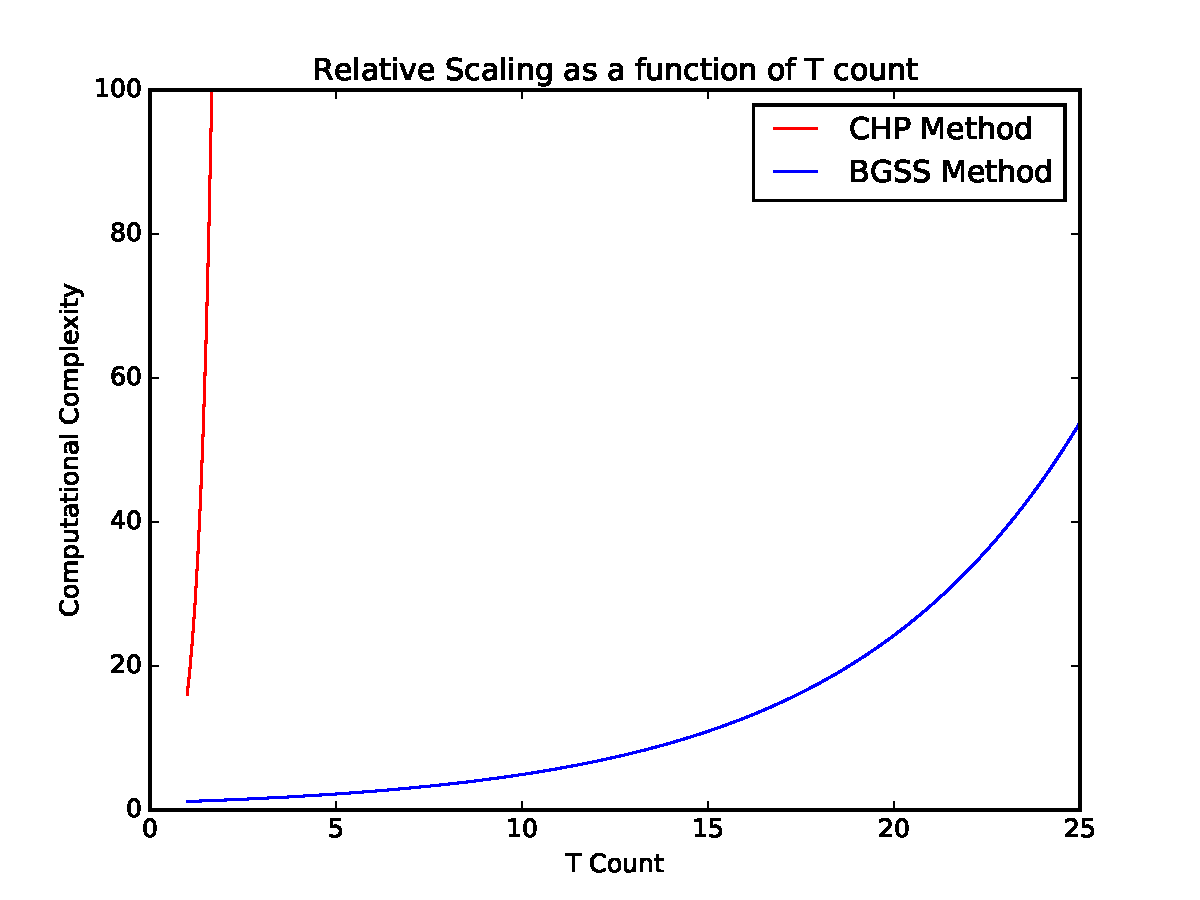
\includegraphics[width=0.6\textwidth]{Figures/tcount.pdf}
\label{fig:quadraticreduction}
\caption{Plot showing the relative behaviour of the dominant exponential scaling factors in the computational complexity for the \texttt{CHP} and \texttt{BGSS} algorithms, simulating a Clifford+T circuit.}
\end{figure}
This indeed seems to be the case; using an implementation of a unitary synthesis algorithm for Clifford+T circuits, I obtained an estimate of 2000 $T$-gates required to realise Shor's algorithm on 10 qubits~\cite{Selinger2012}. Even with the significant reduction in complexity, this would be impractical to simulate using the \texttt{BSSG} method. 
\par
This suggests, then, that the Stabiliser Rank of a given state might instead serve as a useful measure of its value as a quantum computational resource. For example, access to arbitrary quantum states with close to maximal stabiliser rank would imply the ability to implement arbitrary operations, which would definitionally be more efficient in terms of required computtion time and qubits than the restricted set of operations allowed under a faul tolerant scheme. 

\section{Details of the Implementation}
\subsection{Representations of Stabiliser Groups}
\subsection{Computational Complexity}
\ifstandalone
\bibliography{../MResProject.bib,../ManualEntries.bib}
\fi
\end{document}

\chapter{Stabiliser Rank for Alternative Resource States}\label{chap:results}
\documentclass{standalone}
\begin{document}
This interpretation, that the stabilizer rank of a resource state allows us to quantify in some sense its computational power, naturally leads to the question of how the Stabiliser rank scales for alternative resources. \\
Here, we consider single qubit resource states $\ket{R}$, which we use in conjunction with Clifford group operations. The state $\ket{R}$ is an eigenstate of an operator $R\in\mathcal{C}_{n}$, and can be generated by applying a Unitary $U$ to a stabilizer state. We can then show that
\begin{align}\label{eq:resourcegate}
\begin{split}
R\ket{R} &= R U\ket{\phi} : \exists \mathcal{S}_{\phi} \\
U^{\dagger}\ket{R} &= U^{\dagger}U\ket{\phi} = \ket{\phi}\\
\implies UsU^{\dagger} &= R \forall s\in\mathcal{S}_{\phi}\\
&\implies U \in\mathcal{C}_{n+1} \\
\end{split}
\end{align}
As an example, the edge-type magic state $\ket{H}$ is so named as it is an eigenstate of the Hadamard operator $H\in\mathcal{C}_{2}$, and thus the state is generated by a transform $U\in\mathcal{C}_{3}$, and allows us to realise this operation $U$.
\par
In the first section, we will examine Conjecture~\ref{thm:magicrank} made by Bravyi, Smolin \& Smith, by extending their method to find the asymptotic behaviour of $\chi(\ket{F^{\otimes t}})$. \\
We will then use a pair of computational methods, a brute-force search and a proposed resource measure `Robustness', to try and find explicit values of $\chi$ for arbitrary states, magic states, and finally for resource states that would allow us to realise gates from higher levels in the Clifford Hierarchy.

\section{stabilizer rank of the Face States}\label{sec:frank}
The face states are a family of $8$ Clifford-equivalent magic states with a Bloch vector that projects out from the faces on the `simulable' octahedron shown in Fig.~\ref{fig:octahedron}. We will focus on the state $\ket{F}$, which has a description in the computational basis~\cite{Bravyi2005}
\begin{equation}\label{eq:Fstate}
\ket{F} = \cos(\beta)\ket{0}+\mathe^{i\frac{\pi}{4}}\sin(\beta)\ket{1}\;:\;2\beta = \cos^{-1}(\frac{1}{\sqrt{3}}).
\end{equation}
This state is also called $\ket{T}$ in the original paper on magic state distillation~\cite{Bravyi2005}, and $\ket{R}$ by bravyi, Smoilin \& Smith~\cite{Bravyi2015}.
\par
This state is an eigenstate of an operator we shall refer to as $\Delta$, as it is a rotation of the triangular $F$-state face in the octahedron around the axis $\ket{F}$. In particular, it rotates between the states that form the corners of the face.
\begin{align}
\begin{split}
    \Delta\ket{0} &= \ket{+i}\\
    \Delta\ket{+i} &= \ket{+} \\
    \Delta{\ket{+}} &= \ket{0} \\
\end{split}
\end{align}
Because this operator maps stabilizer states to stabilizer states, we can see that it is a Clifford group operation, and thus $\ket{F}$ allows us to realise an operation $U_{F}\in\mathcal{C}_{3}$.
\par
To apply the results of Bravyi \& Gosset discussion in Section~\ref{sec:edgebound}, we need to find a similar expression in terms of $t$-bit strings. As the state is a symmetric point between three stabilizer states, we can define a ternary basis
\begin{align}
\begin{split}
\ket{\tilde{0}} &= \ket{0}\\
\ket{\tilde{1}} &= \ket{+i}\\
\ket{\tilde{2}} &= \ket{+}\\
\end{split}
\end{align}
which has the desired property that each state has the same overlap with $\ket{F}$
\begin{equation}
\left|\braket{\tilde{x}}{F}\right|^{2} = \cos^{2}(\beta)\equiv\mu^{2}.
\end{equation}
\par
Including the relevant phase corrections, we can thus write $t$ copies of the $F$ state as a sum over $t$-bit ternary strings
\begin{equation}
    \ket{F^{\otimes t}} = \frac{1}{(3\mu)^{t}}\sum_{x\in\mathbb{F}_{3}^{t}}\mathe^{i(\vert x\vert_{2}-\vert x\vert_{1})\phi}\ket{\tilde{x}_{1}\otimes\cdots\otimes\tilde{x}_{t}}
\end{equation}
where the angle $\phi$ is equal to $\frac{\pi}{12}$, and $\vert x\vert_{1,2}$ is the $1$ and $2$-weight of the string $x$.\\
This decomposition, however, contains $3^{t}$ stabilizer states, and so is actually over-complete compared to the computational basis representation. 
\par
We thus need a way to define a normalised state associated to linear subspaces $\mathcal{L}\subseteq\mathbb{F}_{3}^{t}$, such that we can find decompositions with $\chi=3^{k}$. This requires redefining the partition function $Z_{F}(\mathcal{L})=\sum_{x\in\mathcal{L}}f(x)$.\\
The additional complication here is the presence of a complex phase in the state. Again, the amplitude of the overlap between the three states is equal
\[\vert\braket{\tilde{x}}{\tilde{y}}\vert = 2^{-\frac{(1-\delta_{xy})}{2}},\]
where $\delta_{xy}$ is the Kronecker delta, but we also have that 
\[
\braket{\tilde{1}}{\tilde{2}}=\frac{1}{\sqrt{2}} 
\mathe^{-i\frac{\pi}{4}} 
= (\braket{\tilde{2}}{\tilde{1}})^*
\]
Thus, the absolute value of the overlap between a pair of strings will have a magnitude given by the difference in their Hamming weights, and an additional correction given by the phases, giving
\begin{equation}
    f(x)\equiv 2^{-\frac{\vert x\vert}{2}}\cos((\vert x\vert_{2}-\vert x\vert_{1})\phi).
\end{equation}
This was verified numerically by calculating the overlap between different linear subspaces. Thus, we can define the appropriate normalised state
\begin{equation}
    \ket{\mathcal{L}}=\frac{1}{\sqrt{3^{k}Z_{F}(\mathcal{L})}}\sum_{x\in\mathcal{L}}
    \mathe^{i(\vert x\vert_{2}-\vert x\vert_{1})\phi}\ket{\tilde{x}_{1}\otimes\cdots\otimes\tilde{x}_{t}}
\end{equation}
\par
Once we have this explicit form for the stabilizer states, we can thus verify a similar form for the overlap between the magic states and a linear subspace
\begin{equation}\label{eq:foverlap}
\vert\braket{F^{\otimes t}}{\mathcal{L}}\vert^{2}=\frac{3^{k}\mu^{2t}}{Z_{F}(\mathcal{L})}.
\end{equation}
which arises from the fact that each bit in each string has overlap $\mu$ with the state $\ket{F}$, and that there are $3^{k}$ such strings, giving 
\[\left|\braket{F^{\otimes t}}{\mathcal{L}}\right|^{2}=\left(\frac{3^{k}\mu^{t}}{\sqrt{3^{k}Z_{F}(\mathcal{L})}}\right)^{2}=\frac{3^{k}\mu^{2t}}{Z_{F}(\mathcal{L})}.\]
\par
We can use this result to prove an equivalent of Lemma~\ref{thm:expectation}. In particular, we need to evaluate the expression
\[\sum_{x\in\mathbb{F}_{3}^{t}\setminus 0^{t}}f(x)\mathbb{E}(\chi_{\mathcal{L}}(x))\] 
The partition function for the string $\ket{\tilde{0}^{\otimes t}}$ is $1$. We can use the fact that $\left|\braket{F^{\otimes t}}{\mathbb{F}_{3}^{t}}\right|^{2}=1$, and rearrange Eq.~\ref{eq:foverlap} to express it in terms of $Z_{F}(\mathcal{L})$, to give
\begin{align}
\begin{split}
\sum_{x\in\mathbb{F}_{3}^{t}\setminus 0^{t}}f(x) &= 
\frac{3^{t}\mu^{2t}}{\left|\braket{F^{\otimes t}}{\mathbb{F}_{3}^{t}}\right|^{2}} - 1\\
&= 3^{t}\mu^{2t}-1
\end{split}
\end{align}
We also note that, as the indicator function $\chi_{\mathcal{L}}(x)$ is 1 if and only if $x\in\mathcal{L}$, and as $\chi_{\mathcal{L}}(0^{t})=1\forall\mathcal{L}$ as the zero-string is the `identity' element for these subspaces, it's expectation value is simply given by
\begin{equation}
\mathbb{E}\left(\chi_{\mathcal{L}}(x)\right)=\frac{3^{t}-1}{3^{k}-1}
\end{equation}
the relative number of elements in the subspace. 
\par
Thus, we can prove that Lemma~\ref{thm:expectation} translates to these linear subspaces on $\mathbb{F}_{3}^{t}$, namely
\begin{equation}
\mathbb{E}\left( Z_{F}(\mathcal{L}) \right)\leq 1+3^{k}\mu^{2t}.
\end{equation}
\par
The subsequent argument given in Eq.~\ref{eq:markovineq}, using Markov's inequality to show that we can find $\mathcal{L}^{\star}:Z\left(\mathcal{L}^{\star}\right)\leq(1+2^{k}\nu^{2t})\left(1+\frac{\delta}{2}\right)$, seems to apply directly for $Z_{f}$ and the linear subspaces on $\mathbb{F}_{3}^{t}$, provided we fix
\begin{align}
\label{eq:fix3k}
9\geq 3^{k}\mu^{2t}\delta\geq 3\\
\label{eq:Zfbound}
\implies\exists\;\mathcal{L}^{\star} : Z_{f}\left(\mathcal{L}^{\star}\right)\leq \left(1+3^{k}\mu^{2t}\right)\left(1+\frac{\delta}{2}\right).
\end{align}
Thus, we can use this inequality on $Z_{f}(\mathcal{L})$ in Eq.~\ref{eq:foverlap}, to show that this state will $\delta$ approximate $\ket{F^{\otimes t}}$.
\begin{align}
\begin{split}
    \left| \braket{F^{\otimes t}}{\mathcal{L}^{\star}}\right|^{2} &\geq
    \frac{3^{k}\mu^{2t}}{\left(1+3^{k}\mu^{2t}\right)\left(1+\frac{\delta}{2}\right)}  \\
    &\geq \frac{1}{\left(1+3^{-k}\mu^{-2t}\right)\left(1+\frac{\delta}{2}\right)}\\
    &\geq \frac{1}{\left(1+\frac{\delta}{2}\right)^{2}} \qquad \text{\small{From Eq.~\ref{eq:fix3k}}}\\
    &\geq 1-\delta \\
\end{split}
\end{align}
This resulting state has a stabilizer rank 
\begin{equation}
\chi=3^{k}\leq 9\mu^{-2t}\delta^{-1} = O\left(\mu^{-2t}\delta^{-1}\right)=O\left(2^{\gamma_{F}t}\delta^{-1}\right)
\end{equation}
where the scaling factor $\gamma_{F}$ is obtained by using the properties of the logarithm to rewrite $\mu^{-2t}=2^{-2t\log_{2}(\mu)}$, giving $\gamma_{F}\approx0.345$.\\
Lemma~\ref{thm:scalinglemma} then follows immediately for the face-type magic states, as it only depends on the maximal value of the overlap between a stabilizer state and the magic state. In this case, it is given by $\mu=\cos(\beta)$, and gives the bound $\chi=\Omega\left(\mu^{-2t}=2^{\gamma_{F}t}\right)$.
\par
Finally, we can consider the problem of approximate computational basis decompositions. The argument given in Equations~\ref{eq:hweight} and~\ref{eq:approxcomp} also applies for our $\ket{F}$ states, but instead is based on the binary entropy $H_{2}(\mu^{2})$. This gives the rank of the approximate computational basis decomposition as
\begin{equation}
    \chi\sim 2^{H_{2}(\mu^{2})}\approx 2^{0.95t}.
\end{equation}
We can check this argument by finding the hamming weight of the computational state with the largest amplitude for a few copies of the states $\ket{F}$, and comparing it to the approximate bound on the maximal Hamming weight given in Eq.~\ref{eq:hweight}. This is shown for up to $\ket{F^{\otimes 16}}$ in Fig.~\ref{fig:compbasis}.
\begin{figure}
    \centering
    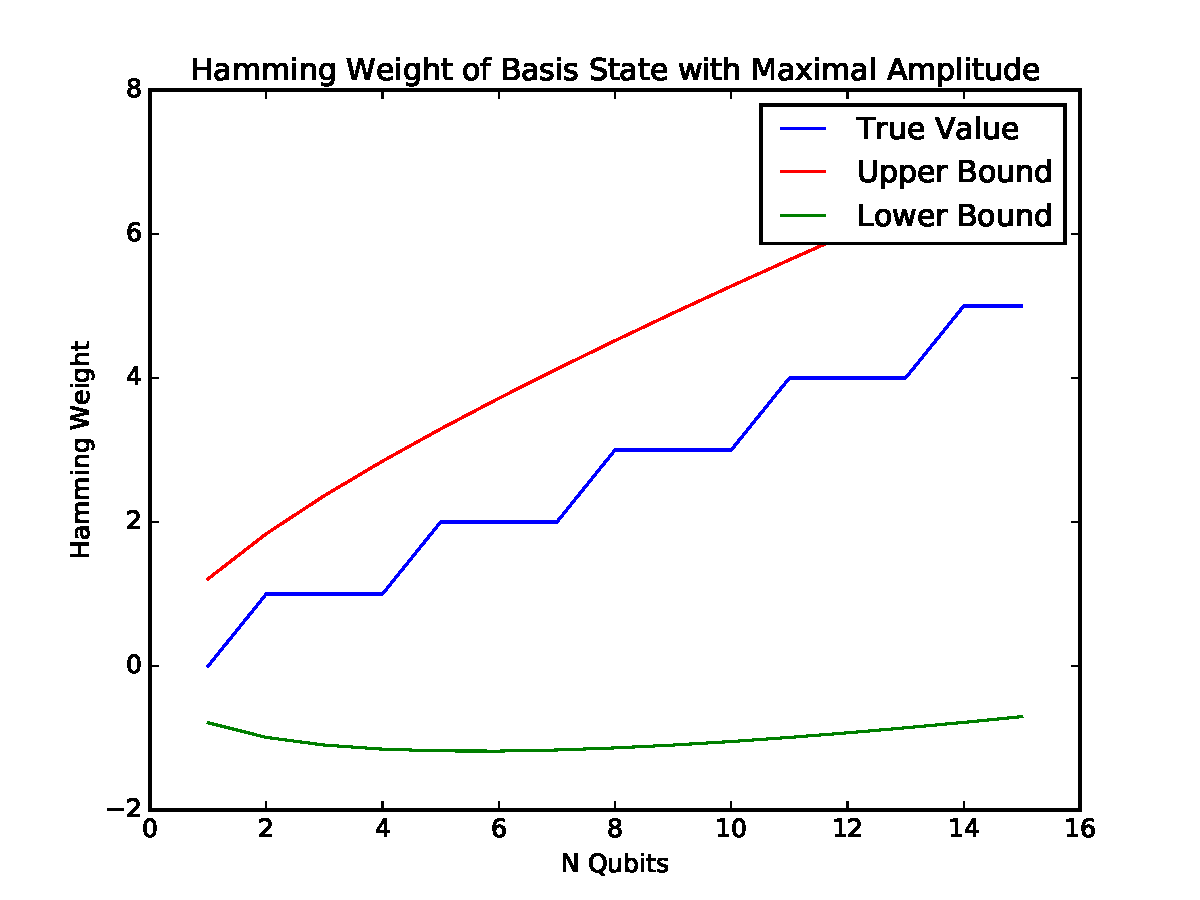
\includegraphics[width=0.7\textwidth]{Figures/computational_bound.pdf}
    \caption{Plot showing the Hamming weight of the computational basis state with the highest amplitude for $n$ copies of the magic states $\ket{F}$, as well as the approximate bounds $\vert x \vert \approx (1-\mu^{2})t\pm O(t)$.}
    \label{fig:compbasis}
\end{figure}

Thus, by defining these approximate decompositions in to ternary strings, we have been able to show that the stabilizer rank of a face-type state has a larger asymptotic bound that for edge-type states. Additionally, if Conjecture~\ref{thm:minscaling} holds, which seems evident from the proof of Lemma~\ref{thm:scalinglemma}, then these states have a stabilizer rank which is strictly larger than for the edge-type states.

\section{Explicit stabilizer rank Decomposition}\label{sec:decompositions}
The technique used above to bound the stabilizer rank of a given state does not easily generalise, because it requires that the state be decomposable into a symmetric superposition of stabilizer states. This is satisfied by magic states, due to their definition as symmetric points between the single-qubit stabilizer states, but doesn't apply for more general resource states. \\
In particular, we would like to analyse the stabilizer rank for resource states that can be used to realise gates from higher levels in the Clifford hierarchy. An easy way to generate such states is to make use of an observation about the Pauli $Z$ operator. By definition as a Pauli operator, $Z$ is in level $\mathcal{C}_{1}$. It's square-root, the Phase gate, is a Clifford operation, and thus $\in\mathcal{C}_{2}$. The root of the phase gate, $T$, is another level higher, $\in\mathcal{C}_{3}$. This seems to suggest that taking repeated roots of the gate $Z$ generators operators from successively higher levels of the Clifford hierarchy. This is indeed the case.
% , which can be verified from the action of these gates on generators of the Pauli group, $X$ and $Z$.
% \par
% The general form of the $n$-th root of a $Z$ gate is
% \begin{equation}
%     Z^{-\frac{1}{n}} = \begin{pmatrix} 1 & 0 \\ 0 & \mathe^{\frac{\mathi\pi}{(n)}} \\ \end{pmatrix} 
% \end{equation}
% which is equal to a pahse gate with angle $\frac{\pi}{n}$, denoted $R_{\frac{\pi}{n}}$. For a Pauli $X$, such a gate acts as 
% \begin{equation}
%     R_{\phi}XR^{\dagger}_{\phi} = \begin{pmatrix}0 & \mathe^{-\mathi\phi} \\ \mathe^{\mathi\phi} & 0 \\ \end{pmatrix}
% \end{equation}
% which is not a Pauli operator for $\phi\notin\{0,\frac{\pi}{2},\pi,\frac{3\pi}{2}$. 
\par
These operators are diagonal and live in $\mathcal{C}_{n\geq3}$, and thus they meet the criteria to be realised using the state injection method discussed in Section~\ref{sec:msi}. This means the corresponding resource state can be generating by acting the operator $Z^{\frac{1}{n}}:n\;\text{mod } 2=0$ on the state $\ket{+}$. \\
However, as these states are given by a rotation of the state $\ket{+}$ by an angle $\phi<\frac{\pi}{2}$ along the equator of the Bloch sphere, they are not symmetric points between pairs of stabilizer states. This means we will need to determine their stabilizer rank explicitly. 
\par
As discussed in Section~\ref{sec:srank}, Brayi, Smolin \& Smith found approximate values for the stabilizer rank of $\ket{H}$ for up to $6$ qubits. They did this by implementing a random-walk within the space of $n$-qubit stabilizer states, seeking to find a decomposition set $\tilde{\phi}:\norm{\Pi_{\tilde{\phi}}\ket{H^{\otimes n}}}=1$~\cite{Bravyi2015}. \par
\begin{algorithm}[!h]
\caption{Random Walk on Stabiliser States}
\label{alg:randwalk}
\begin{algorithmic}[1]
\Require $\beta_{init},\beta_{max},M,$ target integer $\chi$
\State $\tilde{\phi} \leftarrow \left(\phi_{1},\cdots\phi_{\chi}\right)$ where each $\phi_{a}$ is chosen at random.
\State $\beta \leftarrow \beta_{init}$
\While{$\beta < \beta_{max}$}
    \For{$i=0$ to $100$}
        \State Evaluate $F(\tilde{\phi})=1-\norm{\Pi_{\phi}\ket{H^{\otimes n}}}$
        \If{$F(\tilde{\phi})=0$}
            \State \Return $\tilde{\phi}$
        \EndIf
        \State Pick random integer $a$ and random Pauli $P\in\mathcal{P}_{n}$
        \State $\phi_{a}'\leftarrow c\left(\mathbb{I}+P\right)\phi_{a}$
        \State $\tilde{\phi}' \leftarrow (\phi_{1},\cdots,\phi'_{a},\cdots\phi_{\chi})$
        \If{$F(\tilde{\phi}')<F(\tilde{\phi})$}
            \State $\tilde{\phi}\leftarrow\tilde{\phi}'$
        \Else
            \State $p_{accept}\leftarrow \exp[-\beta\left(F(\tilde{\phi}')-F(\tilde{\phi})\right)]$
            \State Pick random $r\in [0,1]$
            \If{$r>p_{accept}$}
                \State $\tilde{\phi}\leftarrow\tilde{\phi}'$
            \EndIf
        \EndIf
    \EndFor
    \State $\beta\leftarrow \beta + \left( \frac{\beta_{max}-\beta_{init}}{M} \right)$
\EndWhile
\State \Return No decomposition found.
\end{algorithmic}
\end{algorithm}
In this algorithm, $\beta$ is a positive-valued parameter analogous to an inverse temperature. This algorithm then resembles a form of Simulated annealing, where we `walk' through an energy landscape defined by the objective function $F$, here given by $1-\norm{\Pi_{\phi}\ket{H^{\otimes n}}}$, trying to find a global minimum, and move `up' the energy landscape with a probability given by the Boltzmann distribution for $\beta$. Increasing $\beta$ amounts to decreasing the temperature, effectively `freezing' our random walk into a local minimum that presumed to be close-to-optimal.
\par
However, we would like to find minimal decompositions deterministically for a small number of qubits to be able to state categorically the relative stabilizer rank of different resource states. We attempt this using two methods: Brute-Force Search, and a resource measure called Robustness.
\subsection{Computationally Generating Stabiliser States}
Both techniques require us to computationally generate the stabilizer states on $n$ qubits. The number of such states grows rapidly in the number of qubits, and is equal to~\cite{Aaronson2004a}
\begin{equation}\label{eq:nstabs}
    N_{\phi}=2^{n}\prod_{k=0}^{n-1}\left(2^{n-k}+1\right).
\end{equation}
To find the states, we must first build all $n$-qubit stabilizer groups, which we can do by finding their sets of $n$ generators. For each group $\mathcal{S}=\langle s_{1},\cdots,s_{n}\rangle$, we can then build a projector on to the stabilizer space~\cite{Gottesman1997}
\begin{equation}\label{eq:stabproj}
    \Pi_{\mathcal{S}} = \prod_{i=1}^{n} \frac{1}{2}\left(\mathbb{I}+s_{i}\right)
\end{equation}
and the corresponding state can be found by finding it's $+1$ eigenstate.
\par
To generate the stabilizer groups, we employed the binary string representation used by Aaronson\& Gottesman, which was described in Section~\ref{sec:CHP}. Namely, a Pauli operator is defined by $2n+1$ bits: $x_{i}:i\in\{1,\cdots,n\}$, $z_{i}:i\in\{1,\cdots,n\}$ and $r$. The global phase is given by $-1^{r}$, and the $i$th operator in the tensor product by the bits $x_{i},z_{i}$. \\
This allows us to efficiently generate all $n$-qubit Pauli operators with real-valued phase by generating the binary strings $B$ for the numbers $0$ to $2^{2n+1}-1$~\cite{Aaronson2004a}.\\
\par
We can try to generate a stabilizer group by picking a set of $n$ strings from this full set, and generating the corresponding linear subspace by combining the strings under binary addition. To be a valid stabilizer state, we must first check that all $n$ strings mutually commute. We note that two $n$-qubit Pauli operators commute if an even number of qubits are acted on by a pair of Pauli operators. Otherwise, the operators anticommute. For example, 
\begin{align*}
\comm{X\otimes\mathbb{I}\otimes X}{Z\otimes\mathbb{I}\otimes Z}= 0\\
\acomm{X\otimes X\otimes X}{Z\otimes Z\otimes Z} = 0. \\
\end{align*}
In this binary representation, the commutativity of two Pauli operators represented by strings $B_{h},B_{i}$ can be efficiently checked by evaluating their symplectic inner product
\begin{equation}\label{eq:sympprod}
    B_{h}\cdot B_{i} \equiv x_{h,1}z_{i,1}\oplus\cdots\oplus x_{h,n}z_{i,n}\oplus z_{h,1}x_{i,1}\oplus\cdots\oplus z_{h,n}x_{i,n}
\end{equation}
where the addition is modulo 2. The corresponding Pauli operators commute if their binary representations have a symplectic inner product of $0$, and anticommute otherwise.\\
To describe a stabilizer space, the subspace then generated by these commuting operators must contain $2^{n}$ elements, which can be used as a way to check candidate spaces. The resulting space also cannot contain the string corresponding to $0\cdots01$, as this element is equivalent to $-1\mathbb{I}$. Any Pauli subgroup containing the element $-1\mathbb{I}$ cannot have be a stabilizer group, as $-\mathbb{I}\ket{\psi}=-\ket{\psi}$. \\
If the resulting group hadn't previously been found, it was then stored. Otherwise, the candidate group was discarded.
\par
In practice, this method found more `unique' stabilizer groups than expected from Eq.~\ref{eq:nstabs}. This was because the technique was identifying as distinct two groups equivalent up to global phase. Instead, we noted that there are $2^{n}$ ways of distributing the phase between the $n$ generators. For example, on two qubits
\begin{align*}
    \mathcal{S}&=\langle s_{1},s_{2}\rangle \\
    &\neq \langle -s_{1},s_{2}\rangle \\
    &\neq \langle s_{1},-s_{2}\rangle \\
    &\neq \langle -s_{1},-s_{2}\rangle. \\
\end{align*}
Thus, we can generate the full set of stabilizer groups but first generating the $\frac{N_{\phi}}{2^{n}}$ groups with all-positive Pauli operators, and then adding phase to the resulting generators `by hand'. This full method is outlined in Algorithm~\ref{alg:gengroups}, and was implemented in Python using \texttt{Qutip}~\cite{Johansson2012} and the \href{https://github.com/ilanschnell/bitarray}{\texttt{bitarray}} library. Due to the large number of such groups, we were only able to generate the stabiliser states for $n\leq 4$ qubits, due to constrains on available memory.
\begin{algorithm}
\caption{Generating $n$ qubit stabilizer groups}
\label{alg:gengroups}
\begin{algorithmic}
\Function{StringsToPauli}{$G$}
    \State $\mathcal{S}\leftarrow\emptyset$
    \For{$g\in G$}
        \State $\mathcal{S}\leftarrow\mathcal{S}\cup \bigotimes_{i=1}^{n} i^{x_{i}\wedge z_{i}}X^{x_{i}}Z^{z_{i}}$ \Comment{where $g = (x_{1}z_{1}\cdots x_{n}z_{n})\in\mathbb{F}_{2}^{2n}$}
    \EndFor
    \State \Return $\mathcal{S}$
\EndFunction
\end{algorithmic}
\begin{algorithmic}[1]
\Require $n$ \Comment{Number of qubits}
\Require \Call{GetEigenstate}{Projector}
\State S $\leftarrow \mathbb{F}_{2}^{n}$, Generators $\leftarrow \emptyset$, States $\leftarrow\emptyset$
\State TotalGenerators $\leftarrow \frac{N_{\phi}}{2^{n}}$ \Comment{where $N_{\phi}$ is defined in Eq.~\ref{eq:nstabs}.}
\While{$|$Generators$|$ < TotalGenerators}
    \State $G = \{g_{1},\cdots,g_{n}\}\subseteq S$
    \If{$\comm{g_{i}}{g_{j}}=0\;\forall\;g_{i},g_{j}\in G$}
        \State $\mathcal{L}\leftarrow \langle g_{1},\cdots,g_{n}\rangle$
        \If{$-\mathbb{I}\in\mathcal{L}$ \textbf{or} $\left|\mathcal{L}\right| \neq 2^{n}$}
            \State Reject candidate
        \EndIf
        \If{$\mathcal{L}\notin$ Generators}
            \State Generators$\leftarrow$ Generators $\cup \{\mathcal{L}\}$
        \EndIf
    \EndIf
\EndWhile
\For{$G\in$ Generators}
    \State $\mathcal{S}$ = \Call{StringsToPauli}{G}
    \State Projector $\leftarrow \prod_{i=1}^{n}\frac{1}{2}\left(\mathbb{I} + s_{i}\right)\quad \forall s_{i}:\mathcal{S}=\langle s_{1},\cdots,s_{n}\rangle$
    \State States $\leftarrow$ states $\cup $ \Call{GetEigenstate}{Projector}
    \For{$\tilde{x}\in\mathbb{F}_{2}^{n}\setminus 0^{n}$}
        \State Projector $\leftarrow \prod_{i=1}^{n}\frac{1}{2}\left(\mathbb{I} + -1^{\tilde{x}_{i}}s_{i}\right)\quad \forall s_{i}:\mathcal{S}=\langle s_{1},\cdots,s_{n}\rangle$
        \State States $\leftarrow$ states $\cup $ \Call{GetEigenstate}{Projector}
    \EndFor
\EndFor
\State \Return States
\end{algorithmic}
\end{algorithm}
\subsection{Brute Force Search}
This is the simplest method of finding a decomposition in to magic states. For a given $n$, we pick a set of $i$ states from the set of all $n$-quit stabilizer states. We then have to build the projector on to the space generated by these states, and test the overlap with the target states $\ket{R^{\otimes n}}$. If it is equal to one, we are done. Else, we continue testing all $i$ states. If this is exhausted, we increment $i$ and resume. This will continue up to $i=2^{n}$, where the method will find the computational basis decomposition and exit. Pseudo-code for the method is given in Algorithm~\ref{alg:brutef}.
\par
The projector onto the space spanned by the Stabiliser states is found using Gram-Schmidt orthogonalization~\cite{Nielsen2000}. This well established technique for building an orthogonal basis for the space spanned by a collection of vectors $\{u\}$. As the Stabiliser states are known to form a mutually unbiased basis~\cite{Howard2013}, this condition is always met for combinations of Stabiliser states. Pseudo-code for the method is shown in Algorithm~\ref{alg:GramSchmidt}.\\
The Gram-Schmidt orthogonalisation procedure was implemented using the \texttt{Numpy} library for fast matrix operations~\cite{VanderWalt2011}.  
\begin{algorithm}
\caption{Gram Schmidt Orthogonalisation}
\label{alg:GramSchmidt}
\begin{algorithmic}
\Function{Projection}{$\ket{u_{i}},\ket{v_{j}}$}
    \State \Return $\frac{\braket{v_{j}}{u_{i}}}{\braket{u_{i}}{u_{i}}}\ket{u_{i}}$
\EndFunction
\end{algorithmic}
\begin{algorithmic}[1]
\Require $\{\ket{v_{1}},\cdots,\ket{v_{k}}\}$ \Comment{Set of $k$ stabilizer states}
\For{$i=1$ \textbf{to} $k$}
    \State $\ket{u_{i}}\leftarrow\ket{v_{i}}$
    \State $j\leftarrow i-1$
    \While {$j>0$}
        \State $\ket{u_{k}} \leftarrow \ket{u_{k}} -$ \Call{Projection}{ $\ket{u_{j}}$, $\ket{v_{i}}$}
        \State $j\leftarrow j-1$
    \EndWhile
    \State $\ket{u_{i}}\leftarrow \frac{1}{\braket{u_{i}}{u_{i}}}\ket{u_{i}}$ \Comment{Ensure normalisation}
\EndFor
\State $A\leftarrow \left(\ket{u_{1}},\cdots\ket{u_{k}}\right)$ \Comment{Matrix with each vector $\ket{u_{i}}$ as column $i$.}
\State \Return $AA^{\dagger}$ \Comment{Projector onto space spanned by the vectors $\ket{u}$.}
\end{algorithmic}
\end{algorithm}

\begin{algorithm}
\caption{Brute Force Search for stabilizer rank}
\label{alg:brutef}
\begin{algorithmic}[1]
    \Require $\Phi$ \Comment{the set of $n$ qubit magic states}
    \Require \Call{GramSchmdit}{$\tilde{\phi}$} \Comment{Implementation of Orthogonalisation}
    \Function{FindChi}{$\ket{\psi}$}
        \For{$i=1$ to $2^{n}-1$}
            \State $\tilde{\phi}=\left(\phi_{1},\cdots,\phi_{n}\right): \phi_{i}\in\Phi\forall\;i$
            \State $\Pi_{\tilde{\phi}}\leftarrow$ \Call{GramSchmidt}{$\tilde{\phi}$}
            \If{$\norm{\Pi_{\tilde{\phi}}\ket{\psi}}$ \textbf{equals} $1$}
                \State \Return $n,\tilde{\phi}$
            \EndIf
            \State $i\leftarrow i+1$
        \EndFor
        \State \Return $2^{n}$, $\tilde{x}$ \Comment{the set of computational basis states on $\mathbb{C}^{2^{n}}$}
    \EndFunction
\end{algorithmic}
\end{algorithm}
\subsection{The Robustness Measure}\label{sec:robustnessmeasure}
Robustness as a resource measure was first defined by Vidal \& Tarrach in 1999~\cite{Vidal1999}. It was proposed as an alternative measure of entanglement that, combined with other metrics like the entanglement entropy, could be used to fully characterise an entangled state. The motivation behind the measure is to quantify how `robust' an entangled state would be to local operations that increase the mixedness of one subsystem~\cite{Vidal1999}.\\
In a resource theory, states or operations are split in to two categories: `free' resources, $\mathcal{P}_{free}$ and `expensive' resources. For example, in entanglement theory separable states are the free resource, and entangled states the expensive resource~\cite{Vidal1999}. This gives the Robustness a clear geometric picture in terms of the set of free resources, as illustrated in Fig.~\ref{fig:robustshapes}.
\par
From the figure, we can see that we define a pair of states at extreme ends of the free resource set. Given this pair of states, the Robustness is then defined as~\cite{Vidal1999}
\begin{equation}\label{eq:robustness}
    \mathcal{R}(\rho)\equiv\min_{\rho_{+},\rho_{-}\in\mathcal{P}_{free}} 2p+1 : \rho = \left(p+1\right)\rho_{+} - p\rho_{-}.
\end{equation}
This resource has the property that it is $1$ for any state that forms a vertex of $\mathcal{P}_{free}$, and that it is subadditive under the combination of systems~\cite{Vidal1999,Howard2016}. The geometric interpretation here is similar to the techniques used to quantify the power of `non-local' correlations in general probabilistic models, where the `free' resource is the polytope defined by strictly local or `classical' correlation~\cite{Acin2006}.
\[\mathcal{R}(\rho_{1}\otimes\rho_{2})\leq \mathcal{R}(\rho_{1})\mathcal{R}(\rho_{2}).\]
\par
\begin{figure}[h]
    \centering
    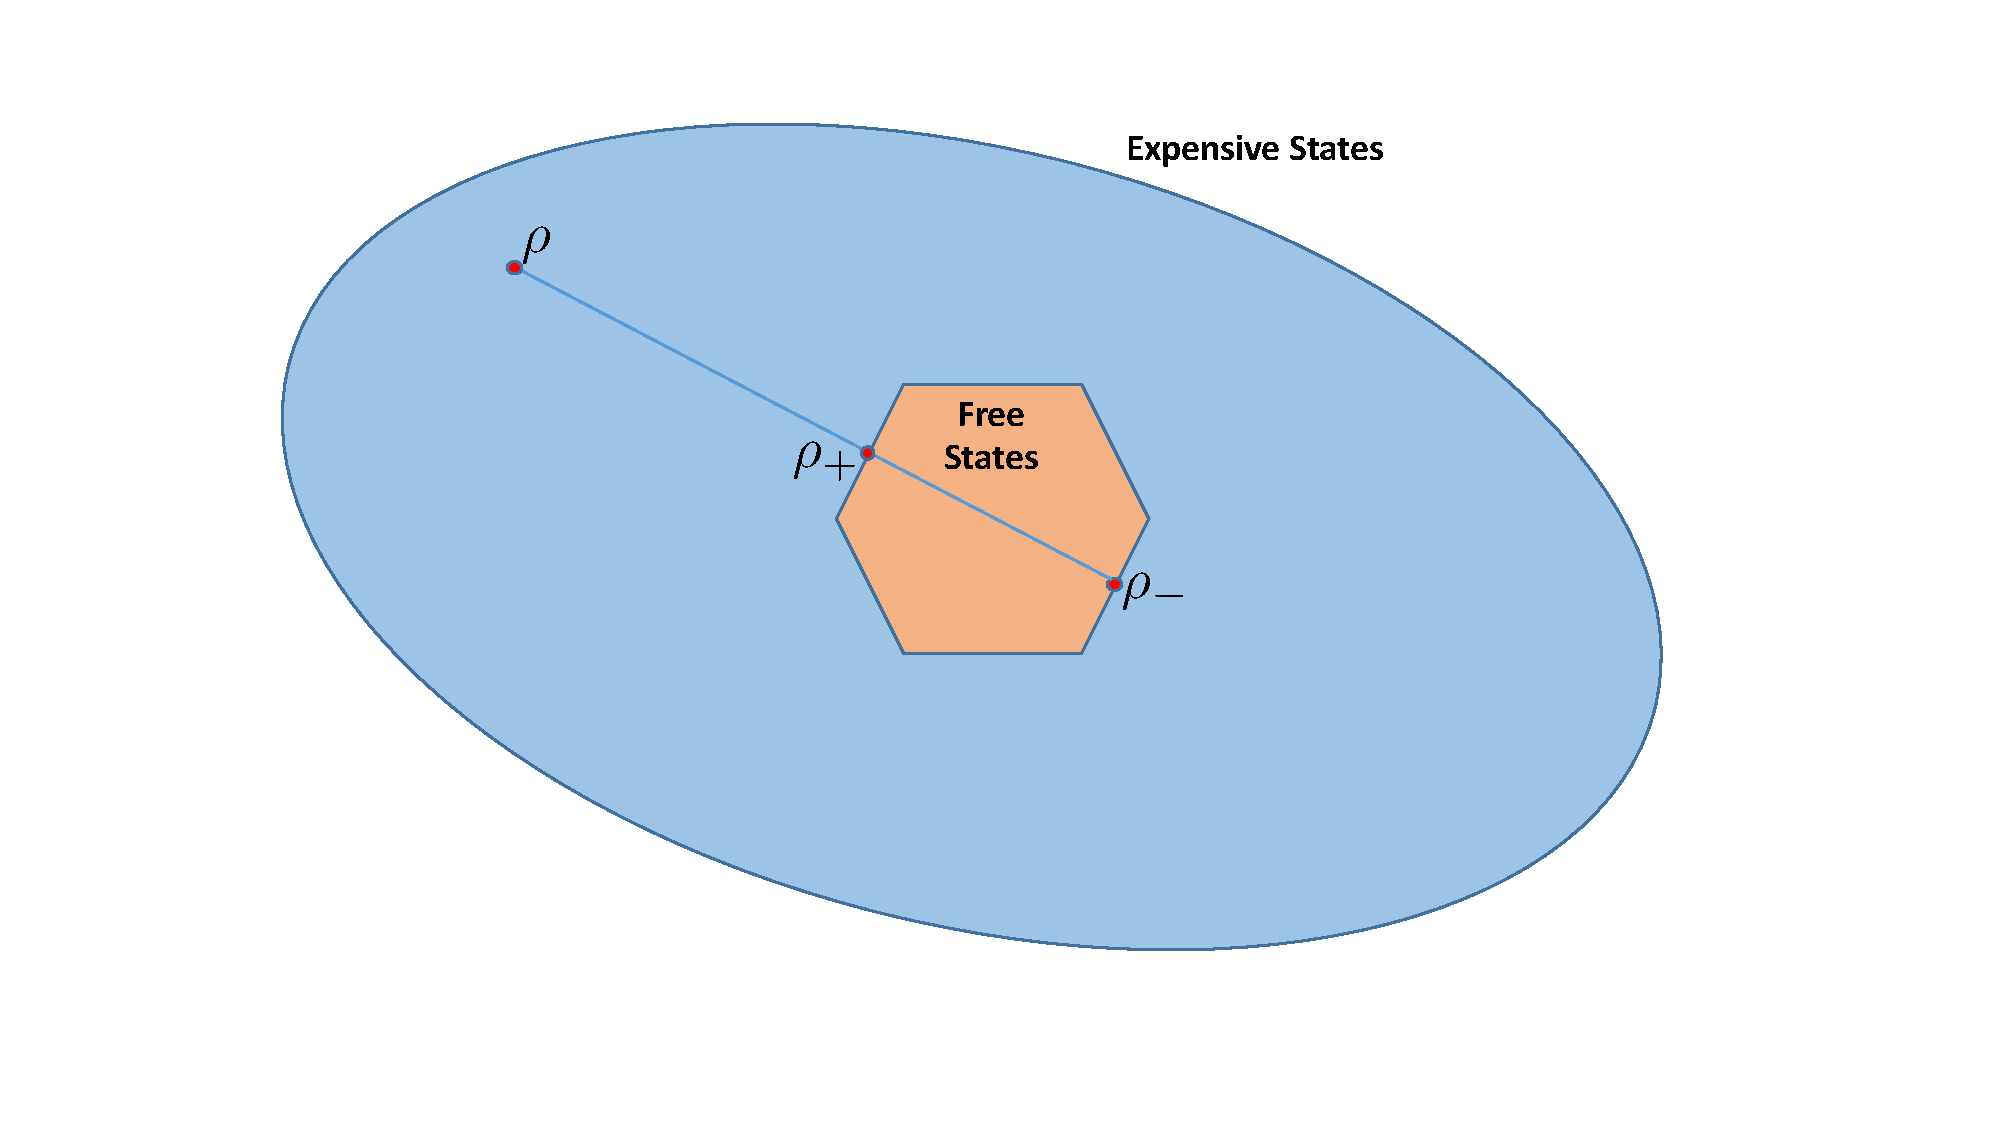
\includegraphics[width=0.6\textwidth]{Figures/Robustness.pdf}
    \caption{Simplified representation of the robustness measure, showing the definition of the vertices $\rho_{\pm}$ relative to the resource state we wish to quantity. Depiction inspired by~\cite{Vidal1999,Howard2016}.}
\label{fig:robustshapes}
\end{figure}
This measure can be adapted to different resource states; in particular, we could consider using it to quantify quantum speedup by defining the free resource as the set of efficiently simulable states, with vertices defined by the stabilizer states. The expensive resource is then the resource states $\ket{R}$ we will use to promote the Clifford circuits to universality~\cite{Howard2016}.\\
The use of Robustness to quantify `magicness' was proposed by Campbell \& Howard~\cite{Howard2016}, motivated by studying contextuality in quantum computing. It is known that for qudits, $d>2$-dimensional quantum states, the onset of Wigner function negativity and contextuality coincide with the definition of magic states. However, qubits display state independent contextuality, and so they sough a measure that would allow them to quantify resource states in qubit and qudit computing. 
\par
It was noted by Campbell \& Howard that the problem of evaluating the Robustness can be converted into a linear programming problem called $\ell_{1}$ minimisation. By defining a matrix $A$ where column $j$ is given by the $j$th vertex of $\mathcal{P}_{free}$. By defining a corresponding column vector $b$ for our resource state, they show that~\cite{Howard2016}
\begin{equation}
    \mathcal{R}(\rho)=\min \norm{x}_{1}\; : Ax=b
\end{equation}
where $\norm{x}_{1}\equiv\sum_{i}\vert x_{i}\vert$.
\par
\begin{algorithm}[t]
\caption{The \texttt{SL0} algorithm for $\ell_{0}$ estimation.}
\label{alg:sl0}
\begin{algorithmic}
\Require $\{\Phi_{i}\}$ \Comment{The set of stabilizer states on a given number of qubits}
\Require SigmaDecreaseFactor \Comment{Authors recommend a value of 0.5~\cite{Mohimani2009}.}
\Require $\mu_{0}$ \Comment{Gradient used in gradient ascent. Authors recommend 2~\cite{Mohimani2009}.}
\Require \Call{PseudoInverse}{Mat} \Comment{Provided by most linear algebra libraries.}
\Function{SmoothedL0}{$n$, $\ket{R}$, $\sigma_{min}$} \Comment{Number of qubits, target state, minimum value of $\sigma$}
    \State $A\leftarrow [A_{i,j}= \braket{i}{\phi_{j}}] \quad \forall\;i\in[0,2^{n}-1], \phi_{j}\in\Phi_{n}$
    \State $b \leftarrow \{b_{i}=\braket{i}{R}\} \quad \forall\;i\in[0,2^{n}-1]$
    \State $A^{+}\leftarrow $ \Call{PseudoInverse}{A}
    \State $x \leftarrow A^{+}b$
    \State $\sigma\leftarrow 2\times \max_{\forall x_{i}\in x} \{\vert x_{i} \vert\}$
    \While{$\sigma > \sigma_{min}$}
        \For{$i=0$ to $i=2$}
            \State $\delta \leftarrow \{f_{\sigma}(x_{i})\;\forall x_{i}\in x\}$
            \State $x\leftarrow x-\mu_{0}\delta$ \Comment{Do the gradient ascent step}
            \State $x \leftarrow x- A^{+}\left(Ax-b\right)$ \Comment{Project $x$ back onto the set of solutions to $Ax=b$~\cite{Mohimani2009}.}
        \EndFor
        \State $\sigma\leftarrow\sigma \times $SigmaDecreaseFactor
    \EndWhile
    \State \Return \Call{CountNonZero}{x}
\EndFunction
\end{algorithmic}
\end{algorithm}
In their talk, Campbell \& Howard noted that for single magic states $\ket{H}$, evaluating a similar problem called $\ell_{0}$ minimisation gave a related measure 
\begin{equation}
    \mathcal{R}'(\rho)=\min \norm{x}_{0}\; : Ax=b
\end{equation}
that corresponded to the value of the Stabiliser rank decomposition $\chi\left(\ket{H}\right)=2$, where $\norm{x}_{0}\equiv \{\# x_{i} : x_{i}\neq 0\}$, the `sparseness' of the vector $x$~\cite{Howard2016}.\\
This can be understood by considering a the explicit construction of the matrix $A$ and vector $b$ in the case where $\mathcal{P}_{free}$ is defined by the set of stabilizer states. In this case, we can define 
\begin{equation}\label{eq:Amat}
    A_{ij}\equiv\braket{i}{\phi_{j}}
\end{equation}
where $\ket{i}$ is the $i$th computational basis state given by the binary representation of the integer $i\in[0,2^{n}-1]$, and $\ket{\phi_{j}}$ is the $j$th Stabiliser state~\cite{Howard2016}. The corresponding definition of $b$ is then
\begin{equation}\label{eq:bvec}
    b_{i}\equiv \braket{i}{R}
\end{equation}
where $\ket{R}$ is the resource state we want to analyse.\\
The vector $x$ thus gives the representation of our state in the stabilizer basis, and the sparsest vector should correspond to the optimal stabilizer rank decomposition. 
\par
It is known that the problem of finding the global minimum of the $\ell_{0}$ norm is $\NP$-hard~\cite{ge2011note}. However, as this problem occurs in a signal processing context, fast heuristic algorithms exist. In particular, we implemented a method called `Smoothed $\ell_{0}$' (\texttt{SL0})~\cite{Mohimani2009}. \\
The \texttt{SL0} algorithm works by using a `gradient ascent' method to approximately maximise a function $f_{\sigma}(x_{i})$ for each element in the vector $x$. This function has the property that
\begin{equation}\label{eq:limf}
    \lim_{\sigma\rightarrow 0}f_{\sigma}(x_{i}) = \begin{cases} 1 & \text{if } x_{i}=0\\
                                                                0 & \text{if } x_{i}\neq 0\\
                                                  \end{cases}
\end{equation}
and so it's maximization for increasingly small values of $\sigma$ should cause us to converge to the sparsest solution of the vector $x$~\cite{Mohimani2009} In particular, they define a Gaussian function~\cite{Mohimani2009}
\begin{equation}\label{eq:fxi}
    f_{\sigma}(x_{i})\equiv x_{i}\exp\left(-\frac{\vert x_{i}\vert^{2}}{2\sigma^{2}} \right).
\end{equation}
Pseudo-code for the \texttt{SL0} method is given in Algorithm~\ref{alg:sl0}. The method was evaluated by building the $A$ matrix for $n$ qubits, and then running \texttt{SL0} using this matrix and the corresponding vector $b$. Correspondence with Stabiliser rank for the single magic state $\ket{H}$ was found using a minimum $\sigma_{min}=1\times 10^{-12}$; further reductions in $\sigma_{min}$ didn't impact the sparseness returned. 
\subsection{Results}
We began by examining the stabilizer rank for arbitrary quantum states, to verify that these $n$-qubit states have a rank $\chi\approx 2^{n}$. The results for both the \texttt{SL0} and brute force searches, are shown in Table~\ref{tab:arbitrary}. We use $\ket{rand_{n}}$ to denote a random state on $n$ qubits, which is distinct from $\ket{rand}^{\otimes n}$, $n$ copies of a given random state.
\begin{table}[!h]
\caption{Stabilizer Rank for arbitrary quantum states}\label{tab:arbitrary}
\centering
\begin{tabular}{||l|c|c|c|c||}
\hline
State & $\ket{rand}$ & $\ket{rand}^{\otimes 2}$ & $\ket{rand_{2}}$ &$\ket{rand}^{\otimes 3}$ \\ \hline
$\norm{x}_{0}$ & 4 & 14 & 15 & 168\\ \hline
Brute Force & 2 & 3  & 4 & $>4$\\ \hline
\end{tabular}
\end{table}\\
We can see that, for the explicit decompositions of $n$ qubit random states, the stabilizer rank is in fact maximal. For multiple copies of a single random qubit, we can see that there is a small reduction in $\chi$; this would be expected from the complexity of the classical description, where a product state requires fewer classical numbers to characterise fully.\\
It is also immediately clear from the results that the \texttt{SL0} method has not successfully converged to an optimally sparse solution, but instead returns an estimate of $\chi$ larger than the simple upper bound given by the computational basis. However, the values returned do seem to be indicative of the magnitude of $\chi$: for example, \texttt{SL0}$(\ket{rand}^{\otimes 2}<$\texttt{SL0}$(\ket{rand_{2}})$.
\par
\begin{table}[!h]
\centering
\caption{Stabiliser Rank for Magic States $\ket{H}$ and $\ket{F}$.}\label{tab:magic}
\begin{tabular}{||l|c|c|c|c||}
\hline
$n$ qubits & $1$ & $2$ & $3$ & $4$ \\ \hline
$\norm{x_{H}}_{0}$ & 2 & 6 & 116 & 3676\\ \hline
$\norm{x_{F}}_{0}$ & 3 & 9 & 108 & 3753\\ \hline
Brute Force H & 2 & 2  & 3 & 4\\ \hline
Brute Force F & 2 & 2  & 3 & $>3$ \\ \hline
\end{tabular}
\end{table}
We can then extend this to examine explicit decompositions for the magic states $\ket{H}$ and $\ket{F}$, which are shown in Table~\ref{tab:magic}. Again, the estimates returned by the \texttt{SL0} method are over-complete, significantly larger than the computational basis decomposition. However, it is interesting to note that the estimates are smaller than the estimates for arbitrary states, and that they are generally larger for the face-type magic states.\\
We can see that the deterministic values of $\chi$ for $\ket{H^{\otimes n}}$ coincide with the approximate values found by Bravyi, Smolin \& Smith~\cite{Bravyi2015}, and given in Table~\ref{tab:approxchi}. Interestingly, the explicit values found for the $\ket{F}$ states coincide with the results for $\ket{H}$, at least as far as $3$ qubits; unfortunately due to the computational time consumed by the brute-force search, the decomposition for the state $\ket{F^{\otimes 4}}$ did not complete in time, so the stabiliser rank given is merely a bound. 
\par

\begin{table}[!h]
\centering
\caption{Stabiliser Rank for $\ket{\sqrt{T}}$, $\ket{\sqrt[4]{T}}$.} \label{tab:highercliff}
\begin{tabular}{||l|c|c|c|c||}
\hline
$n$ qubits & $1$ & $2$ & $3$ & $4$ \\ \hline
$\norm{x_{\sqrt{T}}}_{0}$ & 2 & 14 & 150 & 4487\\ \hline
$\norm{x_{\sqrt[4]{T}}}_{0}$ & 2 & 12 & 173 & 5023\\ \hline
Brute Force $\sqrt{T}$ & 2 & 3  & $>3$ & $>3$\\ \hline
Brute Force $\sqrt[4]{T}$ & 2 & 3  & $>3$ & $>3$\\ \hline
\end{tabular}
\end{table}
Finally, we can consider the results for resource states generating gates from higher levels in the Clifford hierarchy. In particular, we consider the $4$-th and $5$-th roots of the $Z$ gate, which we denote as $\sqrt{T}, \sqrt[4]{T}$ respectively. These gates are equivalent to phase gates $R_{\phi}$ with $\phi=\frac{\pi}{8}$ and $\frac{\pi}{16}$. The corresponding decompositions are shown in Table~\ref{tab:highercliff}. \\
What is interesting is that, both the \texttt{SL0} estimates and the explicit decompositions for these $\mathcal{C}_{n>3}$ resource states are larger than for the magic states. The \texttt{SL0} estimates are actually comparable to those for arbitrary quantum states, and the explicit decompositions are already bigger than for magic states for $n=2$.
\ifstandalone
\bibliography{../MResProject.bib,../ManualEntries.bib}
\fi
\end{document}
\chapter{Significance for Fault Tolerant Quantum Devices}\label{chap:discussion}
\documentclass{standalone}
\begin{document}
% Interested in this interpretation of the Stab Rank as a quantifier of the resource
% Most obvious cross check seems to come from arbitrary states: access to the full state space through arbitrary rotations would be the ideal implementation of quantum computing
% However, Fault Tolerance necessitates that we are constrained in the set of operations and ancillae we use
% In the long run, resource choice will be blurred out
% But for small devices, the resource cost becomes signficant
% PBC outlined in the context of compiling a circuit for a device with a small number of qubits: seems like a huge reduction but really, 100 T-gates doesn't get you all that much!
% Different reource designs could impact how much computing power we get out of early quantum devices
%%%
% Face states: Asymptotic bound is larger, as is the strict lower bound
% Decompositions don't seem all that different but due to the initial slow divergence between the two scalings
% Include plot
% Big issue with the face state is it doesn't work in state injection
%%%
% Cn>3 states seem promising
% Could use simulated annealing to study them furhter
% DO work in state injection
%%%
% In any case, this work is just the beginning
% Any swich in resource state also needs to include circuit synthesis work to understand the saving better
As discussed in Section~\ref{sec:whybgss}, we are interested in understanding the stabiliser rank of a state as a potential quantifier of its value in quantum computation. This correspondence is predicated on the idea of using classical simulation to probe the quantum advantage, motivated by the Church-Turing-Deutsch thesis.\\
As noted by Jozsa \& Linden, however, the classical simulation complexity is strongly representation dependent. Assuming the validity of the thesis, the presence of an efficient classical simulation can be used to categorically rule out quantum speedup, but an inefficient classical description does not guarantee quantum advantage. Nonetheless, we argue that the stabiliser rank has the potential to constraint quantum speedup. Because it focuses on simulating universal quantum computations, we do not expect it to reduce to an efficient simulation. However, it does allow a relatively more efficient classical description of certain resource states, and thus it is interesting to probe the connection between $\chi$ and the value of different resources. 
\par
A simple confirmation of this concept large $T$-counts are required to implement quantum algorithms showing exponential speedup, described in Section~\ref{sec:whybgss}. Alternatively, we have shown in Table~\ref{tab:arbitrary} that these stabiliser decompositions offer little to no computational advantage for arbitrary quantum states; their stabiliser rank $\chi\approx2^{n}$. As previously mentioned, this can be understood as representing the ideal of `perfect' control of a quantum system. Access to arbitrary states suggests the ability to perform arbitrary single and multi-qubit operations with high-fidelity, as opposed to having to build them out of the elements of a universal gate set.\\
A reduction in stabiliser rank for resource states, and subsequently in the simulation complexity of the corresponding Clifford+`R' fault tolerant scheme, then has a natural correspondence to the increase in the number of elementary operations and physical qubits required to realise the same circuit relative to `perfect' control. 
\par
\section{Face-Type Magic States}
Under this interpretation, then, the proof presented in Section~\ref{sec:frank} would suggest that the face-type magic states serve as a stronger resource for quantum computation than the edge-type states, as they admit a smaller reduction in classical complexity. This is in fact congruent with the observation in~\cite{Howard2014} that the face-type states lead to a larger violation of contextuality inequalities than edge type states. This seems to further support the interpretation of contextuality as a resource for quantum computing. \\
The relative size of the scaling factors for the two families of magic states is given by
\begin{equation}
    \frac{\gamma_{F}}{\gamma_{H}} = \frac{\log_{2}\left(\cos(\beta)\right)}{\log_{2}\left(\cos(\frac{\pi}{8})\right)} = \frac{3}{2}
\end{equation}
which has a simple geometric interpretation in terms of the definition of each state: edge-type magic states are symmetric points between a pair of stabiliser states, whereas face-type states are the symmetric point between 3 stabiliser states. This can be seen in Fig.~\ref{fig:octahedron}. 
Interestingly, this ratio of $\frac{3}{2}$ is also the ratio of the \texttt{SL0} estimates of $\chi$ for single-copies of the $\ket{F}$ and $\ket{H}$ states. 
\par
However, despite the demonstration of a larger asymptotic bound, the explicit decompositions found for the two families of states were equal up to $4$ qubits. This is most likely a consequence of the small effect of the scaling factors for small number of qubits. The exponential scaling factors $2^{\gamma t}$ for each family of magic states are plotted in Fig.~\ref{fig:magicscale}. Here, you can see that the initial difference in the stabiliser rank is small, and that the two are approximately equal up to $5$ qubits. Thus, the lack of any apparent difference is a consequence of the computational constraints when finding these decompositions. 
\begin{figure}[t]
\centering
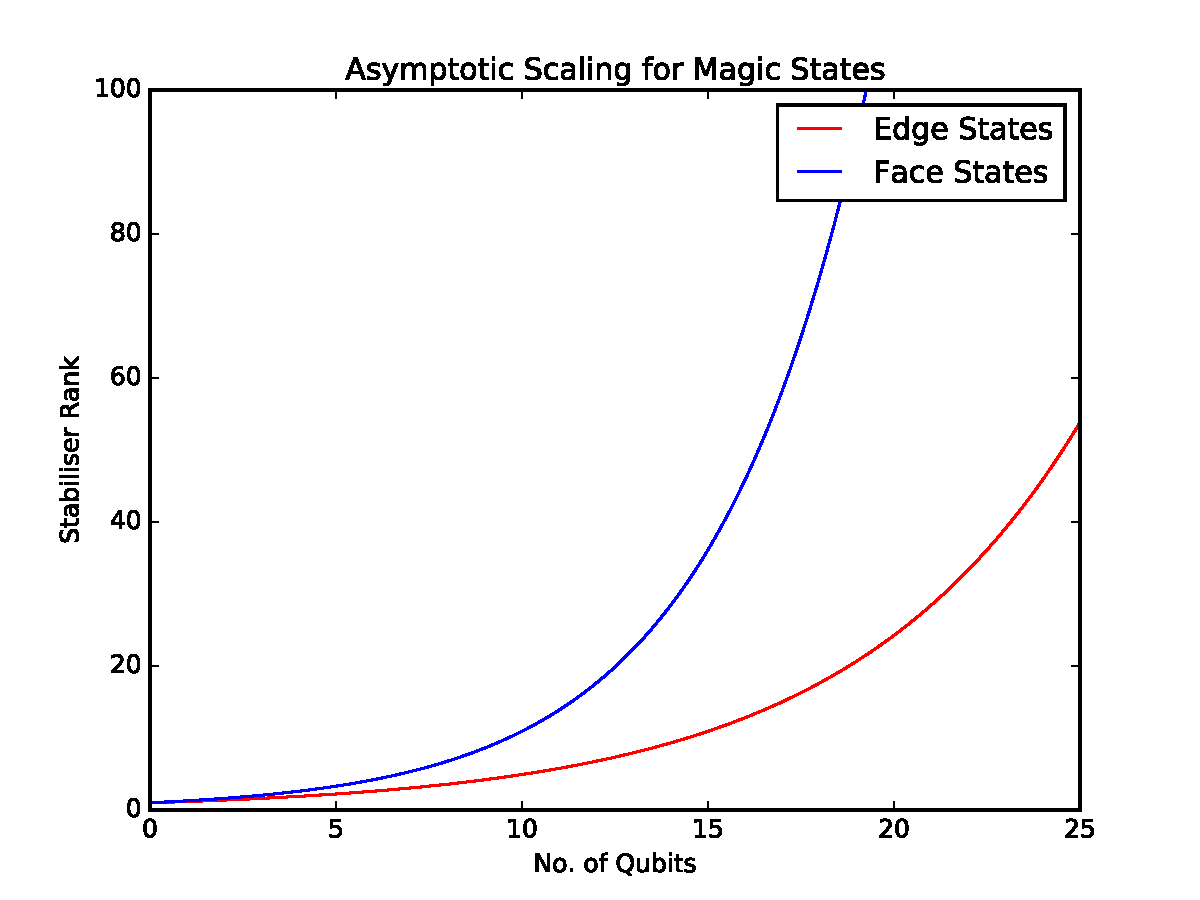
\includegraphics[width=0.75\textwidth]{Figures/magicrank.pdf}
\caption{Plot demonstrating the growth in the exponential scaling factors $2^{\gamma t}$ for both edge and face-type magic states.}
\label{fig:magicscale}
\end{figure}
\par
Unfortunately, a significant reason as to why the quantum computing community focus on the edge-type magic states is that there is currently no known circuit capable of using a face-type state to realise a gate from $\mathcal{C}_{3}$ \emph{deterministically}. The rotation $U:\ket{F}=U\ket{+}$ is equal to a $Y$-rotation followed by a $T$ gate. While demonstrably in $\mathcal{C}_{3}$ from Eq.~\ref{eq:resourcegate}, it is not a diagonal operator and thus the face-type states cannot be used in the state-injection circuit. In their original paper on magic state distillation, Bravyi \& Kitaev demonstrated a circuit that could, probabilistically, convert the state $\ket{F}\otimes\ket{F}$ to a resource state $\ket{A_{\frac{\pi}{6}}}$, that can be used to realise the gate $R_{\frac{\pi}{6}}$~\cite{Bravyi2005}, but no other circuit seems to exist in the literature. 

\section{$\mathcal{C}_{n>3}$ Resource States}
The resource states generated by taking successive roots of the $T$ gate, however, do satisfy the diagonality criteria, and thus can readily be consumed in a state injection circuit. This makes the increase in their stabiliser rank observed already at $2$ qubits especially interesting, as it would suggest that these states are immediately a better candidate resource than either family of magic state. \\
However, this is extrapolating these results from $2$ qubits, and so further research is needed to examine the stabiliser rank of these states. The \texttt{SL0} results seem to suggest a continued growth such that $\chi>\chi_{\text{magic}}$, but the power of this estimator is not well known. Given the seeming accuracy of Algorithm~\ref{alg:randwalk} up to $\ket{H^{\otimes 4}}$, this may serve as a better technique for studying the $\mathcal{C}_{n>3}$ states at higher $n$.

\section{Outlook for Quantum Computing}
As is clear form the case of arbitrary states, and from the lack of a known circuit for employing face-type magic states, a larger stabiliser rank does not immediately translate to a new, stronger resource for fault tolerant quantum computing. \\
There are several related questions that have to be considered when proposing a candidate resource for a Fault Tolerant scheme. Firstly, there is the question of consuming the resource; how readily can we employ it in our computation? 
\par
Secondly, we then have to consider the problem of preparing the resource fault tolerantly. For magic states, distillation schemes have been known and developed since 2005~\cite{Bravyi2005}. In particular, magic state distillation is based on performing stabiliser measurements on multiple, faulty copies, effectively performing quantum error correction to clean up errors in the preparation~\cite{Bravyi2005}. That this technique converges for magic states could perhaps be a direct consequence of their definition as symmetric points on the Bloch sphere between stabilisers.\\
Distillation schemes for alternative resource states are known. The most well developed alternative is Toffoli state distillation and injection, which was first developed by Shor in the earliest proposals on fault tolerant computing~\cite{Shor96}. In general, however, these Toffoli distillation schemes are slightly more resource intensive than magic state distillation~\cite{Eastin2013}. Most modern fault-tolerant proposals instead build a Toffoli gate in a circuit consuming $4-5$ magic states~\cite{Howard2016}. There seems to be a connection, then, between the computational power of the Toffoli gate (equivalent to several $T$ gates) and the resources required to distil the corresponding ancilla. This suggests that distillation schemes for alternative resource states likely exist, but that they may not be as efficient as magic state distillation. 
\par
The final question we have to consider is the problem of circuit synthesis: what are the resources required to implement a given computation in our chosen universal gate set? Current circuit synthesis techniques are best developed for the Clifford+T basis. There is known universal result, the Solovay-Kitaev theorem, for generating any arbitrary unitary in any gate set, but the resulting circuit complexity is known to be well in excess information theoretic bounds. Thus, the question of what resources different Clifford+R schemes require to implement a given computation remains open.\\
Come indications come from current fault-tolerant schemes, which require a certain number of $T$ gates to realise other unitary operations, such as the Toffoli example given above, but it is not yet known if these realisations are optimal. 
\par
When continued development in scalable qubit manufacturing and control allows us to build increasingly large quantum devices, these difference in resource costs will become less and less important; we will have sufficiently large physical resources that any universal construction will be realisable. However, in the near term, the resource costs represent a significant hurdle. \\
The PBC model of computing was derived by Bravyi, Smolin \& Smith in the context of trying to compile a quantum computation for implementation on a small quantum device with a fixed number of qubits, $O(10^{2})$. Initially, it might seem that the reduction of the circuit to a measurement on $t$ magic states represents a significant resource saving. But the rapid growth in the T-count of a circuit already discussed reveals the challenge of choosing a weak universal gate set. The seemingly minimal stabiliser rank of the edge-type magic states, and the existence of circuits requiring multiple $T$ gates to implement other useful $\mathcal{C}_{3}$ gates, does suggest that the Clifford+T basis is perhaps the most resource intensive choice for a universal fault tolerant design. Thus, the problem of developing alternative fault tolerant schemes becomes the problem of extracting as much computational power as possible from our early quantum devices. 
\ifstandalone
\bibliography{../MResProject.bib,../ManualEntries.bib}
\fi
\end{document}
\chapter*{Conclusion}\label{chap:conclusion}
\documentclass{standalone}
\begin{document}

In this report, we have discussed the role of classical descriptions and simulations of quantum mechanics as a tool to try and understand the origins of quantum speedup. In particular, we focused on a novel simulation technique developed by Bravyi, Gosset, Smolin \& Smith. \\
This technique does not admit an efficient classical simulation of quantum computation, which is believed to be impossible. Instead, it is able to significantly reduce the classical complexity of simulating quantum circuits built using the Clifford+T gate set. This particular gate set lies at the heart of modern schemes for fault tolerant quantum computation.
\par
This reduction in complexity derives from the decomposition of the edge-type magic states used to realise T gates into a sum of $\chi$ stabilizer states, where $\chi$ is called the stabilizer rank. The stabilizer rank seems to be minimal for these edge-type states; combined with existing observations about the T-count of other quantum gates, and the stabilizer rank of arbitrary quantum states, we argue that computational savings achieved by the stabilizer rank method are related to the value of the state as a resource for fault tolerant computing.\\
Given this interpretation, we examined the behaviour of the stabilizer rank for alternative resource states: the class of face-type magic states, and resource states for gates in higher levels of the Clifford hierarchy. 
\par
The results seem to confirm that the edge-type magic states have the smallest stabilizer rank, and imply that there could be an advantage to building a fault tolerant scheme around alternative resource states, including gates from $\mathcal{C}_{n>3}$. Further work on adapting circuit synthesis techniques for different universal gate sets would be required to extend these results to give clear proposals for building quantum devices. 

\section*{Future Work}
These results, especially concerning $\mathcal{C}_{n>3}$ resource states, are preliminary, mostly due to computational constraints in finding the stabilizer rank decompositions with the brute-force search methods. The numerical techniques employed thus need further development. 
\par
The programme used to find the stabilizer states could be significantly improved in several ways. The simplest point is an implementation detail: rewriting the programme in \texttt{C} would allow finer memory management, reducing the footprint of the programme. \\
A more significant improvement would be to use an alternative representation of the stabilizer states, that does not require building the Pauli operators in each group and explicitly solving for the corresponding $+1$ eigenstate. This representation extends the use of binary subspaces on $\mathbb{F}_{2}^{n}$ to include binary quadratic functions~\cite{Dehaene2003}. It can then be shown that a stabilizer state is characterised by a linear subspace $\mathcal{L}\subseteq \mathbb{F}_{2}^{n}$, a quadratic function $q:\mathbb{F}_{2}^{n}\rightarrow\mathbb{F}_{2}$ and a `shift' vector $t\in\mathbb{F}_{2}^{n}$~\cite{Dehaene2003,Gross2007}. This is in fact the computational representation used by Bravyi \& Gosset in their implementation of the stabilizer rank method. Combined with a better method of generating these linear subspaces than brute-force search, this would allow stabilizer states to be generated much more efficiently. \\
Alternatively, given the good correspondence between the simulated annealing method and brute-force up to 4 qubits, switching to a simulated annealing search would allow the numerical analysis to be extended. The significant advantage here is that we only need to be able to generate $\chi$ unique, random $n$-qubit stabilizer states, rather than the full set. The other points in the phase space are then generated by applying Pauli operators to random states in the decomposition set $\tilde{\phi}$, as outlined in Algorithm~\ref{alg:randwalk}.
\par
Extending the technique used by Bravyi \& Gosset to bound the stabilizer rank beyond magic states would also allow us to find asymptotic bounds for the rank of the $\mathcal{C}_{n>3}$ states, to compliment further numerical work. 
\par
It would also be useful to understand the computational complexity of determining the stabilizer rank of a given state. This problem is evidently in $\NP$, as any candidate decomposition can be checked in polynomial time by building the projector and evaluating the overlap. \\
There is also an indication that the problem is $\NP$-hard. For example, finding the sparsest vector $x:Ax=b$ is known to be $\NP$-hard~\cite{ge2011note}. Setting $b$ as the computational basis representation and $A$ as the transformation between the computational and stabilizer state bases, as constructed in Section~\ref{sec:robustnessmeasure}, makes finding the sparsest solution $x$ equivalent to finding $\chi$. An alternative proof strategy could be based on the known $\NP$-hardness of finding sparse decompositions of doubly-stochastic matrices~\cite{Dufosse2016}.
\par
Finally, it would also be interesting to improve on the use of the \texttt{SL0} method to estimate the stabilizer rank. While the $\ell_{0}$ minimization problem is known to be $\NP$-hard, the related $\ell_{1}$ problem is in fact solvable exactly~\cite{Howard2016}. It is also known that under certain conditions, the global minima of the $\ell_{1}$ and $\ell_{0}$ problems coincide~\cite{Sawada2005}. Thus, it would be interesting to see if this heuristic can be used to solve for stabilizer rank by calculating the $0$-norm of solutions found using $\ell_{1}$ minimization techniques. 

\section*{Acknowledgements}
I would like to thank my supervisor Dr. Dan Browne for his discussions and input throughout the project, and Dr. Mark Howard for sharing his slides on the robustness measure for quantifying `magicness'. I would also like to thank the staff and students of the EPSRC CDT in Delivering Quantum Technologies for their training and support. 

\ifstandalone 
\bibliography{../MResProject.bib,../ManualEntries.bib}
\fi
\end{document}
\bibliographystyle{nicebib}
\bibliography{../MResProject.bib,../ManualEntries.bib}
\end{document}
%%%༼ つ ◕_◕ ༽つ P R A I S E ~ L a T e X ༼ つ ◕_◕ ༽つ%%%